\documentclass[
10pt, % Main document font size
a4paper, % Paper type, use 'letterpaper' for US Letter paper
oneside, % One page layout (no page indentation)
%twoside, % Two page layout (page indentation for binding and different headers)
headinclude,footinclude, % Extra spacing for the header and footer
BCOR5mm, % Binding correction
]{scrartcl}

\usepackage{listings}
\usepackage{color}
%\usepackage{biblatex}

\definecolor{dkgreen}{rgb}{0,0.6,0}
\definecolor{gray}{rgb}{0.5,0.5,0.5}
\definecolor{mauve}{rgb}{0.58,0,0.82}

\lstset{frame=tb,
	language={},
	aboveskip=3mm,
	belowskip=3mm,
	showstringspaces=false,
	columns=flexible,
	basicstyle={\small\ttfamily},
	numbers=none,
	numberstyle=\tiny\color{gray},
	keywordstyle=\color{blue},
	commentstyle=\color{dkgreen},
	stringstyle=\color{mauve},
	breaklines=true,
	breakatwhitespace=true,
	tabsize=3
}

\usepackage{german}


%usepackage[utf8]{inputenc}
%\usepackage{geometry}
\usepackage[german,onelanguage,linesnumbered, ruled]{algorithm2e}
\SetAlFnt{\small}
\SetAlCapFnt{\large}
\SetAlCapNameFnt{\large}
%\usepackage{algpseudocode}


%%%%%%%%%%%%%%%%%%%%%%%%%%%%%%%%%%%%%%%%%
% Arsclassica Article
% Structure Specification File
%
% This file has been downloaded from:
% http://www.LaTeXTemplates.com
%
% Original author:
% Lorenzo Pantieri (http://www.lorenzopantieri.net) with extensive modifications by:
% Vel (vel@latextemplates.com)
%
% License:
% CC BY-NC-SA 3.0 (http://creativecommons.org/licenses/by-nc-sa/3.0/)
%
%%%%%%%%%%%%%%%%%%%%%%%%%%%%%%%%%%%%%%%%%

%----------------------------------------------------------------------------------------
%	REQUIRED PACKAGES
%----------------------------------------------------------------------------------------

\usepackage[
nochapters, % Turn off chapters since this is an article        
beramono, % Use the Bera Mono font for monospaced text (\texttt)
eulermath,% Use the Euler font for mathematics
pdfspacing, % Makes use of pdftex’ letter spacing capabilities via the microtype package
dottedtoc % Dotted lines leading to the page numbers in the table of contents
]{classicthesis} % The layout is based on the Classic Thesis style

\usepackage{arsclassica} % Modifies the Classic Thesis package

\usepackage[T1]{fontenc} % Use 8-bit encoding that has 256 glyphs

\usepackage[utf8]{inputenc} % Required for including letters with accents

\usepackage{graphicx} % Required for including images
\graphicspath{{Figures/}} % Set the default folder for images

\usepackage{enumitem} % Required for manipulating the whitespace between and within lists

\usepackage{lipsum} % Used for inserting dummy 'Lorem ipsum' text into the template

\usepackage{subfig} % Required for creating figures with multiple parts (subfigures)

\usepackage{amsmath,amssymb,amsthm} % For including math equations, theorems, symbols, etc

\usepackage{varioref} % More descriptive referencing

%----------------------------------------------------------------------------------------
%	THEOREM STYLES
%---------------------------------------------------------------------------------------

\theoremstyle{definition} % Define theorem styles here based on the definition style (used for definitions and examples)
\newtheorem{definition}{Definition}

\theoremstyle{plain} % Define theorem styles here based on the plain style (used for theorems, lemmas, propositions)
\newtheorem{theorem}{Theorem}

\theoremstyle{remark} % Define theorem styles here based on the remark style (used for remarks and notes)

%----------------------------------------------------------------------------------------
%	HYPERLINKS
%---------------------------------------------------------------------------------------

\hypersetup{
%draft, % Uncomment to remove all links (useful for printing in black and white)
colorlinks=true, breaklinks=true, bookmarks=true,bookmarksnumbered,
urlcolor=webbrown, linkcolor=RoyalBlue, citecolor=webgreen, % Link colors
pdftitle={}, % PDF title
pdfauthor={\textcopyright}, % PDF Author
pdfsubject={}, % PDF Subject
pdfkeywords={}, % PDF Keywords
pdfcreator={pdfLaTeX}, % PDF Creator
pdfproducer={LaTeX with hyperref and ClassicThesis} % PDF producer
} % Include the structure.tex file which specified the document structure and layout

\hyphenation{Fortran hy-phen-ation} % Specify custom hyphenation points in words with dashes where you would like hyphenation to occur, or alternatively, don't put any dashes in a word to stop hyphenation altogether

%----------------------------------------------------------------------------------------
%	TITLE AND AUTHOR(S)
%----------------------------------------------------------------------------------------

\title{\normalfont\spacedallcaps{Projektaufgabe AE}} % The article title

\subtitle{Remove Duplicates - Spotify playlist cleaner} % Uncomment to display a subtitle

\author{\spacedlowsmallcaps{Raphael Drechsler}} % The article author(s) - author affiliations need to be specified in the AUTHOR AFFILIATIONS block

\date{} % An optional date to appear under the author(s)

%----------------------------------------------------------------------------------------

\begin{document}

%----------------------------------------------------------------------------------------
%	HEADERS
%----------------------------------------------------------------------------------------

\renewcommand{\sectionmark}[1]{\markright{\spacedlowsmallcaps{#1}}} % The header for all pages (oneside) or for even pages (twoside)
%\renewcommand{\subsectionmark}[1]{\markright{\thesubsection~#1}} % Uncomment when using the twoside option - this modifies the header on odd pages
\lehead{\mbox{\llap{\small\thepage\kern1em\color{halfgray} \vline}\color{halfgray}\hspace{0.5em}\rightmark\hfil}} % The header style

\pagestyle{scrheadings} % Enable the headers specified in this block

%----------------------------------------------------------------------------------------
%	TABLE OF CONTENTS & LISTS OF FIGURES AND TABLES
%----------------------------------------------------------------------------------------

\maketitle % Print the title/author/date block

\setcounter{tocdepth}{2} % Set the depth of the table of contents to show sections and subsections only

\tableofcontents % Print the table of contents

%\listoffigures % Print the list of figures

%\listoftables % Print the list of tables




%----------------------------------------------------------------------------------------

\newpage % Start the article content on the second page, remove this if you have a longer abstract that goes onto the second page

%----------------------------------------------------------------------------------------
%	INTRODUCTION
%----------------------------------------------------------------------------------------
\section{Problemstellung ''Remove Duplicates''}

\textbf{Problem}\\
Gegeben ist eine Sequenz. Diese Sequenz enthält ggf. Duplikate. \\
Ziel des umzusetzenden Algorithmus ist das Entfernen der Duplikate aus dieser Sequenz.\\

Für die Umsetzung eines entsprechenden Algorithmus sollen die zwei folgenden Ansätze betrachtet werden:
\begin{itemize}[noitemsep]
	\item Naiver Ansatz: Nutzung eines einfachen Arrays
	\item Ansatz im Fokus: Nutzung einer Hash-Table
\end{itemize}\

\textbf{Naiver Ansatz}\\
In der Implementierung nach dem naiven Ansatz würden alle Daten einer Sequenz in einem Array gespeichert werden, insofern sie nicht bereits im Array enthalten sind. Beim betrachten eines Elementes aus der Sequenz muss also in der naiven Umsetzung das komplette Array nach einem identischen Element durchsucht werden. Im in Hinblick auf die Laufzeit schlimmsten Fall, muss daher jedes Element im Array mit dem aktuell untersuchten Element des Sequenz verglichen werden. Bei einer Sequenz-Liste der Größe \(n\) müssen also im wors-case 
\begin{equation}
	\sum_{k=1}^{n-1} k
\end{equation}
Vergleichsoperationen durchgeführt werden. Betrachtet man die folgende Umformung entsprechend der Gaußschen Summenformel
\begin{equation}
	\sum_{k=1}^{n-1} k = \frac{(n-1)^2 + (n-1)}{2} = \frac{1}{2} (n-1)^2
\end{equation}


ergibt sich für eine Umsetzung dieses Ansatzes eine theoretische obere Komplexitätsgrenze von 

\begin{equation}
O(n^2)
\end{equation}


\textbf{Ansatz Hash-Table}\\
Der Ansatz ''Hash-Table'' setzt an dem Punkt der Komplexitätsbetrachtung an\\
Würde man für die Einordnung der Elemente in das Array eine Direktadressierung verwenden, so würde man ein Element selbst als Schlüssel interpretieren, mit dem ein Feld im Array adressiert wird.

\begin{figure}[h]
	\centering 
	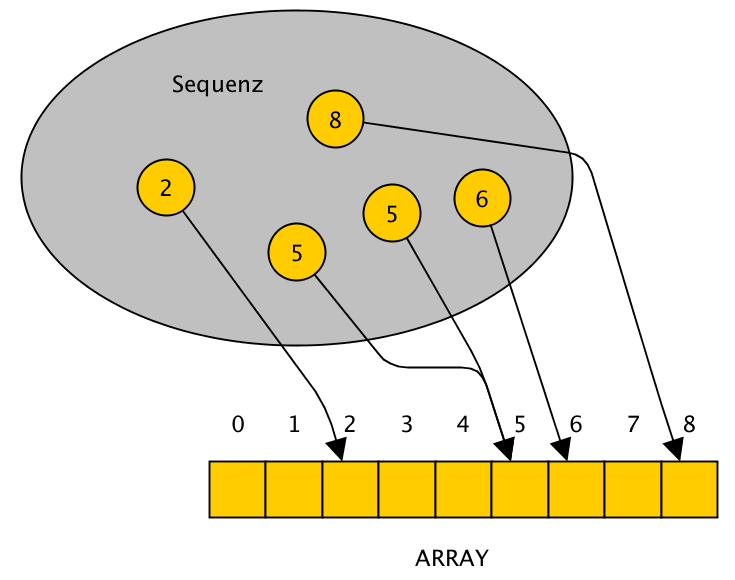
\includegraphics[width=0.5\columnwidth]{Diag1} 
	\caption[Skizze Direkte Adressierung]{Skizze: Prinzip der direkten Adressierung \textit{nach} \cite{Cormen:2009:IAT:1614191}}
	
\end{figure}

Der Zeitaufwand für die Prüfung, ob ein Element bereits im Array gespeichert ist, wäre dabei \(O(1)\).\\
Ist das Universum \(U={0,1,...,m}\), in denen sich die Schlüssel der Elemente befinden klein, lässt sich somit schnell auf ein Array der Größe \(A[0..m-1]\) zugreifen. Ab einer bestimmten Größe des Universums kann eine Umsetzung der Direkt-Adressierung Aufgrund der erforderlichen Größe des Ziel-Arrays nicht mehr sinnvoll bzw. möglich sein.\\
Die Hash-Table löst dieses Problem, indem sie das große Universum \(U\) einem kleineren Array \(A[0..m-1]\) gegenüberstellt. Die Adressierung der Array-Felder pro Element erfolgt weiterhin auf Grundlage des Element-Wertes. Um nur existierende Schlüssel zu erhalten wird zur Ermittlung des Schlüssels eine Funktion \(h\) (sogenannte Hash-Funktion) eingesetzt, welche die Werte der Elemente im Universum \(U\) auf existierende Schlüssel abbildet. \textit{vgl.}\cite{Cormen:2009:IAT:1614191}
\begin{equation}
h: U-> {0,...,m-1}
\end{equation}\
Die Skizze gestaltet sich wie folgt:\\
\begin{figure}[h!]
	\centering 
	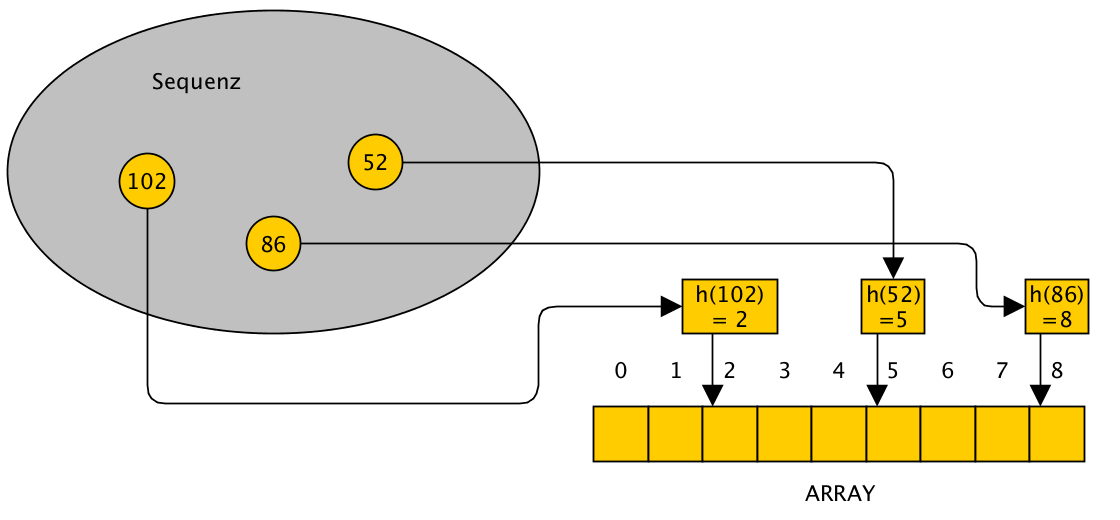
\includegraphics[width=0.75\columnwidth]{Diag2} 
	\caption[Skizze Adressierung in Hash-Table]{Skizze: Prinzip der Adressierung in einer Hash-Table\textit{nach} \cite{Cormen:2009:IAT:1614191}}
	
\end{figure}\

Dadurch, dass gilt \(|U|>m\) wird über Anwendung des Schubfachprinzips ersichtlich, dass die Hash-Funktion \(h\) nicht injektiv ist. \\
Fälle in denen gilt
\begin{equation}
h(a)=h(b)|a,b\in U, a\neq b
\end{equation}
werden als Kollision bezeichnet. \textit{vgl.}\cite{Cormen:2009:IAT:1614191}\\
Bei der Umsetzung des Algorithmus muss also eine entsprechende Strategie zur Auflösung solcher Kollisionen mit betrachtet werden.\\

\textbf{Kollisions-Auflösung im python dict-Objekt}\\
Als Kollisions-Auflösungs-Strategie soll im Rahmen der Umsetzung das Verfahren implementiert werden, welches im python-Standard beim Zugreifen auf \textit{dict}-Objekte genutzt wird. Durch die ggf. notwendige Behandlung von Kollisionen ergibt sich für einen Zugriff auf ein Feld des Arrays bei einer entsprechenden Implementierung der folgende Zeitbedarf.

\begin{table}[h!]
	\centering 
	\begin{tabular}{|l|c|c|c|c|c|}
		\hline 
		Operation & average-case & worst-case \\ 
		\hline 
		Element einfügen & \(O(1)\) & \(O(n)\)\\
		\hline 
		Auf Element zugreifen & \(O(1)\) & \(O(n)\)\\
		\hline 
	\end{tabular}\\
	\caption[Zugriffs-Komplexität im python dict]{Zugriffs-Komplexität im python dict \cite{TimeComplexityPy}}
\end{table}\

\section{Anwendungsszenario Spotify Playlists}
Als Anwendungsfall soll das disjunkte Vereinigen von Titeln mehrerer Spotify-Playlists betrachtet werden.\\
In Spotify lassen sich für eine geöffnete Playlist per Tastatur-Kurzbefehl ''Strg + A'' und ''Strg + C'' alle Titel der Playlist in die Zwischenablage kopieren. Die Titel werden dabei als URI repräsentiert.

\begin{figure}[h!]
	\centering 
	\begin{lstlisting}
	https://open.spotify.com/track/757530vPBymdi31CtXstxP
	https://open.spotify.com/track/1Qi256uJuMihknGuuFcQoC
	https://open.spotify.com/track/0JFBf2PloRfMkPg5DjXhDx
	https://open.spotify.com/track/7iXF2W9vKmDoGAhlHdpyIa
	\end{lstlisting}
	\caption[Beispiel Spotify-Titel URIs]{Beispiel: Spotify-Titel URIs}
\end{figure}\

Die URIs werden durch den Anwender in einem separatem \textit{.txt}-File gesammelt. Somit werden mehrere Playlists in diesem \textit{.txt}-File vereinigt.\\
Die Bereinigung der Duplikate soll nun der zu implementierende Algorithmus übernehmen.\\
Nach Abschluss der Bereinigung lassen sich alle URIs des \textit{.txt}-Files in die Zwischenablage kopieren und per Tastatur-Kurzbefehl ''Strg + V'' in Spotify in eine (sinnvollerweise neue) Playlist einfügen.

\section{Funktionsweisen der Algorithmen}
Im Rahmen der Lösungs-Umsetzung des ''Remove Duplicates''-Problems sollen drei verschiedene Implementierungen in der Sprache python betrachtet werden.\\
Dabei soll das Hauptaugenmerk auf der ersten Implementierung liegen. Diese soll die Funktionalität der \textit{dict}-Objekte in python nachempfinden, indem Sie die entsprechende hash-Funktion und die entsprechende Kollisions-Auflösungs-Strategie implementiert.\\
Zum Vergleich sollen zwei weitere Implementierungen betrachtet werden:\\
\begin{itemize}[noitemsep]
	\item der in Kapitel 1 beschriebene naive Ansatz 
	\item eine Lösung, welche die tatsächlichen python \textit{dict}-Objekte nutzt
\end{itemize}\
Im Folgenden werden die Implementierungen mittels Pseudo-Code beschrieben.

\subsection{Funktionsweise Haupt-Algorithmus: dict-like}

Zunächst wird eine hash-table in Form eines Arrays initialisiert.\\

\textbf{Haupt-Algorithmus: Hash-Tabelle initialisieren}\\
 \begin{algorithm}[H]
	\KwResult{$table$, $tableSize$}
	$tableSize \leftarrow$ 8;\\
	$table \leftarrow$ Array der Größe $tableSize$;\\
	
\end{algorithm}\

Anschließend werden die Elemente (URIs) aus der Sequenz-Datei des Nutzers in die angelegte hash-table geschrieben. Tritt dabei ein Element doppelt auf, wird dieses als Duplikat erkannt und ignoriert.\\
Als hash-Funktion wird dabei die python-Standardfunktion \textit{hash()} eingesetzt. Die Strategie zur Kollisionsauflösung entspricht derjenigen, die bei python \textit{dict}-Objekten Anwendung findet und lässt sich dem folgenden Pseudocode entnehmen.

\textbf{Haupt-Algorithmus: Elemente in Array einfügen}\\
\begin{algorithm}[H]
	\SetKwRepeat{Do}{tue}{solange}
	\KwData{$Sequenz-Datei$}
	\KwResult{$table$}
	\For{Jede $URI$ in $Sequenz-Datei$}{
		$index \leftarrow$ \(hash(\)$URI$\()\);\\
		$uriHandled \leftarrow flase$;\\
		$pertub \leftarrow None$;\\
		\Do{$! uriHandled$}{
			\uIf{bereits Element in $table[index]$ enthalten}{
				\uIf{$table[index] == URI$}{
					//Duplikat liegt vor - $URI$ wird ignoriert\\
					$uriHandled \leftarrow true$;\\
				}
				\Else{
					\uIf{$pertub$ besitzt Wert}{
						$pertub = pertub >> 5$;\\
						$index \leftarrow ((5*slotindex)+1+pertub) \% tableSize$;\\ 
					}
					\Else{
						$pertub = index$;\\
					}
				}
			}
			\Else{
				$table[index] \leftarrow $ $URI$;\\
				$uriHandled \leftarrow true$;\\
			}
		}
		\uIf{URIs in $table$ > \(\frac{2}{3}*\) $tableSize$}{
			\Do{$4 * |$URIs in $table |$ \(>=\) $tableSize$}{
				$tableSize \leftarrow tableSize * 2 $
			}
			$newTable \leftarrow table$;\\
			Kopiere alle URIs in $table$ unter Errechnung neues Schlüssels in $newTable$;\\
			$table \leftarrow newTable$;\\
		}
	}
\end{algorithm}\

Anschließend werden die in der hash-table enthaltenen URIs in eine Output-\textit{.txt}-Datei geschrieben. Diese enthält damit die Duplikat-freie Liste der URIs und kann vom Anwender genutzt werden.

\subsection{Funktionsweise Vergleichs-Algorithmus 1: Naiver Ansatz}
Der in Kapitel 1 skizzierte naive Ansatz gestaltet sich grundlegend wie folgt.\\
\textbf{Algorithmus Naiver Ansatz}\\
\begin{algorithm}[H]
	\KwData{$Sequenz-Datei$}
	\KwResult{$table$}
	$table \leftarrow []$;\\
	\For{Jede $URI$ in $Sequenz-Datei$}{
		$uriInTable \leftarrow false$;\\
		\For{Jede $processedUri$ in $table$}{
			\uIf{$processedUri == URI$}{
				$uriInTable \leftarrow true$;\\
			}
		}
		\uIf{$uriInTable$}{
			//Duplikat erkannt, ignoriere es\\
		}
		\Else{
			$table.append(URI)$;\\
		}
	}
\end{algorithm}\

Anschließend erfolgt die Ausgabe der Duplikat-freien Liste per Erzeugen einer Output-Datei.


\subsection{Funktionsweise Vergleichs-Algorithmus 2: python dict}
Die Funktionsweise des zweiten Vergleichs-Algorithmus ist diejenige, deren Verhalten in der Umsetzung des Haupt-Algorithmus angestrebt wird.\\
Folglich zeichnet sich der Quellcode der Implementierung durch die Nutzung von python-Standard-Operatoren aus. Der wesentliche Teil der Implementierung umfasst die folgenden Zeilen Code:\\
\lstinputlisting[language=python]{pyCode1.py}
Analog zu den anderen zwei Implementierung erfolgt im Anschluss eine Ausgabe aller Elemente des dicts per Output-File.\\


Alle drei initialen Implementierungen finden sich im Abgabeordner unter \textit{/Code/02\_ImplementierungOhneVerbesserung}.
Zum Aufruf der Algorithmen über die Kommandozeile muss die zu untersuchende \textit{.txt}-Datei als Parameter angegeben werden. Beispielhaft sei hier ein Aufruf der ersten Implementierung gezeigt.

\lstinputlisting[language=sh]{call1.sh}


\section{Messdaten}
Zur Beschaffung von möglichst großen und verschiedenen Playlists als Messdaten wurde zunächst ein Test-Daten-Generator implementiert. Dieser wird in 4.1 näher beschrieben.\\
Im Folgenden wurde ein kurzes Programm implementiert, welches die Spotify Web-API nach Titeln anfragt und somit echte Datensätze erhält. Dieser Echt-Daten-Abgreifer wird in 4.2 näher beschrieben.\\
Zudem wurde für das Durchführen von Messreihen mit wachsender Playlist-Größe ein Vorgehen etabliert, um die benötigten .txt-Files zu erzeugen. Dieses wird in 4.3 erläutert.

\subsection{Test-Daten-Generator}

Der Aufruf des Generators erfolgt mit zwei optionalen Parametern und einem obligatorischem Parameter.
\begin{lstlisting}
testDataGenerator.py <n> [dupFactor] [fileSuffix]
\end{lstlisting}
Der Parameter \textit{n} entspricht der Anzahl der Elemente, welche die zu generierende Liste enthalten soll. Der \textit{dupFactor} entspricht der Wahrscheinlichkeit mit der ein Element in der Liste ein Duplikat ist. Der \textit{fileSuffix} kann bei mehreren ausgegebenen Dateien mit gleicher Parametrisierung für eine unterschiedliche Benennung genutzt werden.\\ 
Ein Beispiel für einen Aufruf könnte wie folgt aussehen.\\
\lstinputlisting[language=sh]{call2.sh}

Im Wesentlichen erzeugt der Test-Daten-Generator eine \textit{.txt}-Datei im sequence-File-Format. Die dynamischen Teile der URIs, (welche einen base62-Code \cite{SptfyTrackID} der Länge 22 darstellen) werden dabei zufällig erzeugt und ergeben im Regelfall keine tatsächlich existierende URI.\\
Die Funktionsweise des Generators ist dabei wie folgt zu beschreiben. \\

\textbf{Algorithmus Test-Daten-Generator}\\
\begin{algorithm}[H]
	\KwData{$n, [dupFactor],[fileSuffix]$}
	\KwResult{$.txt-File$}
	\uIf{$dupFactor$ nicht gegeben}{
		$dupFactor \leftarrow$ zufälliger Faktor aus $\{$\(0.0,0.1,...0.9\)$\}$;\\
	}
	$linkList \leftarrow []$;\\
	\For{$i$ in $\{0,...,n-1\}$}{
		\uIf{$i>0$}{
			\uIf{Zufallsentscheidung mit Wahscheinlichkeit $dupFactor = positiv$}{
				$linkList.append(linkList[i-1])$;\\
			}
			\Else{
				$linkList.append($neue zufällige URI$)$;\\
			}
		}
		\Else{
			$linkList.append($neue zufällige URI$)$;\\
		}
	}
	erzeuge neues $.txt-File$ ggf mit Suffix $fileSuffix$;\\
	Schreibe in 1. Zeile von $.txt-File$ ''$secquenceString$'';\\
	Schreibe Elemente aus $linkList$ in Zufalls-Reihenfolge in $.txt-File$;\\
\end{algorithm}\

Die resultierende Datei \textit{(Beispielsweise ''generatedTestData100000\_0.4dupFac\_Run1.txt'')} ist dann bereit zur Verarbeitung durch einen implementierten Algorithmus oder lässt sich zum Erstellen mehrerer Playlist für eine Messreihe einsetzen. \textit{(Siehe 4.3)}\\

Die Implementierung des Algorithmus findet sich im Abgabeordner unter \textit{Code/01\_Daten\_Generieren/01\_TestDaten/testDataGenerator.py}.

\subsection{Echt-Daten}
Für das Beschaffen von großen Playlists mit echten Track-URIs wurde eine Java-Anwendung umgesetzt, welche mithilfe eines Wrappers \cite{API} die Spotify API abfragt.\\
Um eine beliebig große Menge an URIs abzufragen, wurden das unten dargestellte Vorgehen für das Abfragen der API implementiert. Dabei müssen eine Mindest-Anzahl an URIs, die erhalten werden sollen und die URI eines Interpreten als Start-Interpreten angegeben werden.\\

Der entsprechende Java-Projektordner findet sich im Abgabeordner unter \textit{Code/01\_Daten\_Generieren/02\_EchtDaten/realDataGetter}.

\textbf{Algorithmus Echt-Daten-Abgreifer}\\
\begin{algorithm}[H]
	\SetKwRepeat{Do}{tue}{solange}
	\KwData{$minimalNoOfUris, startArtist$}
	\KwResult{$outputFile.txt$}
	Autorisierungsprozess zwischen Anwendung und Spotify API;\\
	$outputTracklist \leftarrow []$;\\
	$searchProcessedArtists \leftarrow []$;\\
	$searchUnprocessedArtists \leftarrow []$;\\
	$processedArtists \leftarrow []$;\\	
	$searchUnprocessedArtists.add(startArtistUri)$;\\
	\Do{$|outputTracklist|<=minimalNoOfUris$ UND $searchUnprocessedArtists$ ist nicht leer}{
		\For{$artist$ in $api.getRelatedArtists(searchUnprocessedArtists.get(0))$}{
			\uIf{$artist$ nicht in $processedArtists$}{
				$searchUnprocessedArtists.add(artist);$
				\For{$album$ in $api.getAlbumsForArtist(artist)$}{
					\For{$track$ in $album$}{
						$outputTracklist.add(track)$;\\
					}
				}
			$processedArtists.add(artist)$;\\
			}
		}
	$searchProcessedArtists.add(searchUnprocessedArtists.get(0))$;\\
	$searchUnprocessedArtists.remove(0)$;\\
	}
	Erzeuge $outputFile.txt$;\\
	Schreibe in Zeile 1 von $outputFile.txt$ ''secquenceString'';\\
	\For{$URI$ in $outputTracklist$}{
		Schriebe $URI$ in $outputFile.txt$;\\
	}	
\end{algorithm}\

Analog zu 4.1 kann die generierte Datei im Anschluss verarbeitet werden.

\subsection{Skalieren der Daten-Listen}
Um später ganze Messreihen auszuführen, bei denen die Anzahl der Elemente, die in den Playlists enthalten sind, im Verlaufe der Messreihe zunimmt, wurde ein python-Skript erstellt, welches ein Sequenz-File einliest und nach eine Neue Datei erstellt, welche nur die Anzahl an Zeilen (zuzüglich der Zeile ''secquenceString'') beinhaltet, welche als zweiter Parameter übergeben wird.

Der Aufruf erfolgt beispielsweise wie folgt:
\lstinputlisting[language=sh]{call3.sh}

Um viele Dateien für eine Messreihe zu generieren, wird ein kurzes shell-Skript je Messreihe angepasst und anschließend eingesetzt.\\

Das python- und das shell-Skript finden sich im Abgabeordner unter\\ \textit{Code/01\_Daten\_Generieren/03\_DatenSkalieren}.

\section{Vorbereiten der Messungen}
Bevor der die Algorithmen-Laufzeiten untereinander und mit den jeweiligen theoretischen Laufzeiten verglichen werden, soll zunächst das Profiling und das Optimieren der einzelnen Implementierungen erfolgen. (Kapitel 5.1 - 5.3)\\
Die Vorbereitung der Messungen wird mit Kapitel 5.4 abgeschlossen, in dem beleuchtet wird, welche Messungen auf welche Weise erfolgen.

\subsection{Profiling und Optimierung Haupt-Algorithmus}
Generell soll für die Laufzeit-Messungen nur das Abarbeiten der Track-URIs, also das schreiben dieser in die hash-table bzw. das dict im Fokus stehen. Daher werden für alles Weitere die Funktionalitäten für das Schreiben des Ergebnis-Files auskommentiert.\\
Für den Hauptalgorithmus liegt die entsprechende \textit{.py}-Datei im Abgabeordner unter \textit{Code/03\_Messen\_und\_Verbessern/01\_Alg\_1/1\_dictLike\_improvement0.py}.\\

Für das Profiling wird ein mittels \textit{testDataGenerator.py} erstelltes \textit{.txt}-File mit Größe \(n=100.000\) und der Duplikat-Wahrscheinlichkeit von \(dupFac = 2\%\) verwendet.\\
Das Profiling erfolgt über die Nutzung des python-Profilers \textit{cProfile} \cite{CPROF}.\\

Die erste Visualisierung des Profils mittels \textit{Snakeviz}\cite{SNAKE}zeigt:\\
\begin{figure}[h!]
	\centering 
	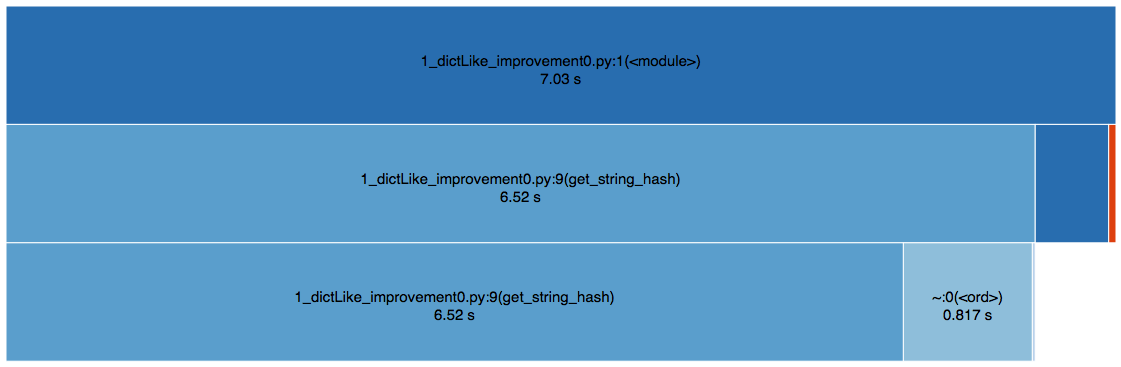
\includegraphics[width=0.75\columnwidth]{pro1} 
	\caption[Darstellung initiales Profiling Alg. 1]{Darstellung initiales Profiling von Algorithmus 1}
\end{figure}\

Die Funktion \textit{get\_string\_hash} macht einen Großteil der Arbeitszeit aus. Diese Funktion ist der python-Standard-Funktion \textit{hash()} nachempfunden. Das Implementieren dieser Funktion sollte dem tieferen Verständnis dienen.\\
Die wesentliche Verbesserung besteht also im ersetzten der \textit{get\_string\_hash}-Funktion durch den python-Standard.\\
Der angepasste Algorithmus ist im Abgabeordner unter\\ \textit{Code/03\_Messen\_und\_Verbessern/01\_Alg\_1/1\_dictLike\_improvement1.py} enthalten.\\
\begin{figure}[h!]
	\centering 
	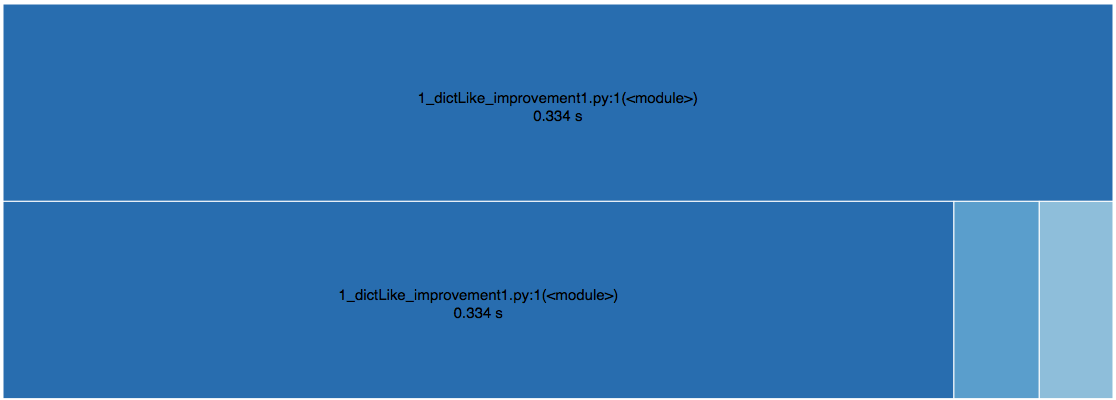
\includegraphics[width=0.75\columnwidth]{pro2} 
	\caption[Darstellung Profiling Alg. 1 nach 1. Verbesserung]{Darstellung Profiling von Algorithmus 1 nach 1. Verbesserung}
\end{figure}\

Würde man diesem Prinzip der Optimierung folgen, also alles, wofür es python-Standard-Funktionalitäten gibt mit python-Standard-Funktionalitäten lösen, so würde der auf diesem Wege final optimierte Algorithums zu dem zweiten Vergleichs-Algorithmus (Kapitel 3.3.) identisch sein.\\
Daher soll im nächsten Schritt einer potentiellen Verbesserung das Tailoring angesetzt werden.\\

Betrachtet man die URIs, wird klar, dass die hash-Funktion nur auf den 22-stelligen Base62-Code angewendet werden muss, da der restliche Teil für alle URIs identisch ist.\\
\begin{lstlisting}
https://open.spotify.com/track/757530vPBymdi31CtXstxP
https://open.spotify.com/track/1Qi256uJuMihknGuuFcQoC
\end{lstlisting}

Der entsprechend angepasste Algorithmus ist im Abgabeordner unter\\ \textit{Code/03\_Messen\_und\_Verbessern/01\_Alg\_1/1\_dictLike\_improvement2.py} enthalten. Die Ausgabe-Funktion muss für eine Anwendung um den statischen Teil der URIs erweitert werden. Dies wurde in der Datei, obgleich die Ausgabefunktion für die Messungen auskommentiert bleibt, getan.\\

Da die Profile bezüglich ihrer gesamt benötigten Laufzeit für einen sichtbaren Unterschied zu nahe beieinander lagen, wurde das Profiling der vorherigen Version \textit{1\_dictLike\_improvement1.py} und das Profiling der Verbesserten Variante mit einem \textit{.txt}-File der Größe \(n=1.000.000\) wiederholt.

Die Verbesserung ist marginal. Bei mehrfachem Messen zeigte sich, dass durch Schwankungen anhand Gesamt-Laufzeit nicht erkannt werden konnte welche Implementierung schneller ist. Durch das Profiling jedoch stellte sich heraus, dass die benötigte Zeit für das Anwenden der Hash-Funktion bei in jedem Profil für den zweiten Algorithmus geringer war, weshalb die Anpassung im Rahmen des Tailorings als sinnvoll anerkannt und beibehalten werden kann.


\begin{table}[h!]
	\centering 
	\begin{tabular}{|l|c|c|c|c|}
		\hline 
		Durchlauf & Vor Tailoring gesamt & Nach T. gesamt & Vor T. hash() & Nach T. hash()\\ 
		\hline
		1	& \(2,65s\)	& \(2,54s\)	& \(0,185s\) & \(0,143s\) \\
		\hline
		2	& \(2,61s\)	& \(2,62s\)	& \(0,183s\) & \(0,146s\) \\
		\hline
		3	& \(2,74s\)	& \(2,43s\)	& \(0,188s\) & \(0,138s\) \\
		\hline
	\end{tabular}\\
	\caption[Ergebnisse Tailoring]{Ergebnisse des Tailorings: Benötigte Zeit gesamt und für hash-Funktion}
\end{table}\

Abschließend seien hier die Zeitbedarfe für je einen Durchlauf einer Verbesserungs-Stufe des ersten Algorithmus für die oben verwendete Playlist mit \(n=100.000\) Elementen dargestellt:

\begin{figure}[h!]
	\centering 
	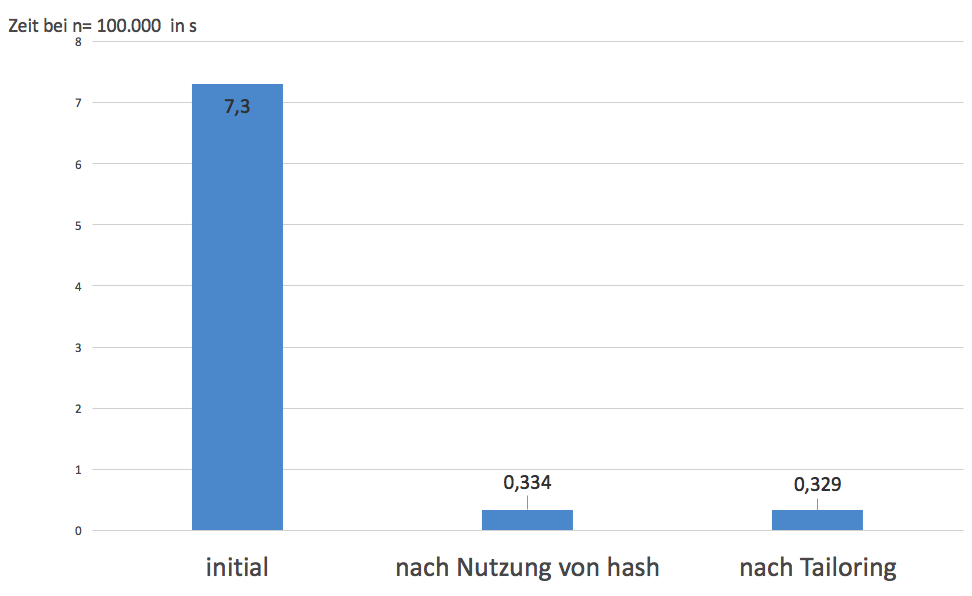
\includegraphics[width=0.75\columnwidth]{pro1fin} 
	\caption[Zusammenfassung Optimierung Alg. 1]{Zusammenfassung der Optimierung von Algorithmus 1}
\end{figure}\

\subsection{Profiling und Optimierung Vergleichs-Algorithmus 1}
Analog zu der in Kapitel 5.1 gewonnenen Erkenntnis, soll die Verbesserung des Algorithmus in zwei Schritten ablaufen:
\begin{enumerate}[noitemsep]
	\item Ersetzen von implementierten Funktionalitäten, die mit python-Standards gelöst werden können (Iterieren durch Array ablösen durch Verwendung des \textit{in}-Operators)
	\item Anpassen des Algorithus analog zum in 5.1 durchgeführten Tailoring
\end{enumerate}\

Die entsprechenden Implementierungen sind im Abgabeordner unter\\ \textit{Code/03\_Messen\_und\_Verbessern/02\_Alg\_2/} enthalten.\\

Die zusammengefasste Verbesserung gestaltet sich für ein Beispiel der Laufzeit mit \(n=10.000\) für Algorithmus 2 wie folgt:\\
\begin{figure}[h!]
	\centering 
	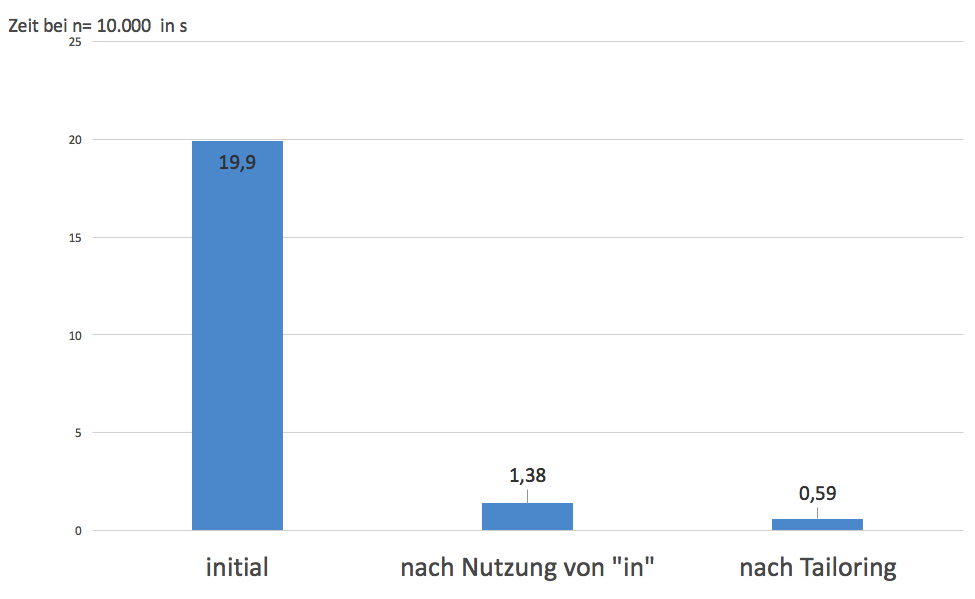
\includegraphics[width=0.75\columnwidth]{pro2fin} 
	\caption[Zusammenfassung Optimierung Alg. 2]{Zusammenfassung der Optimierung von Algorithmus 2}
\end{figure}\

Die Verbesserung ist ähnlich zu der in Kapitel 5.1 erzielten, wobei jedoch das Tailoring für Algorithmus 2 eine größere Wirkung zeigt.

\subsection{Profiling und Optimierung Vergleichs-Algorithmus 2}
Da in dieser Umsetzung bereits die python-Standardfunktionen genutzt werden, soll hier nur das Tailoring betrachtet werden. Die entsprechenden Implementierungen sind im Abgabeordner unter \textit{Code/03\_Messen\_und\_Verbessern/03\_Alg\_3/} enthalten.\\

Die Verbesserung wird erst ersichtlich, wenn man die Anzahl der URIs in der Liste deutlich erhöht. Ab \(n=10.000.000\) zeigt sich der Effekt:\\
\begin{figure}[h!]
	\centering 
	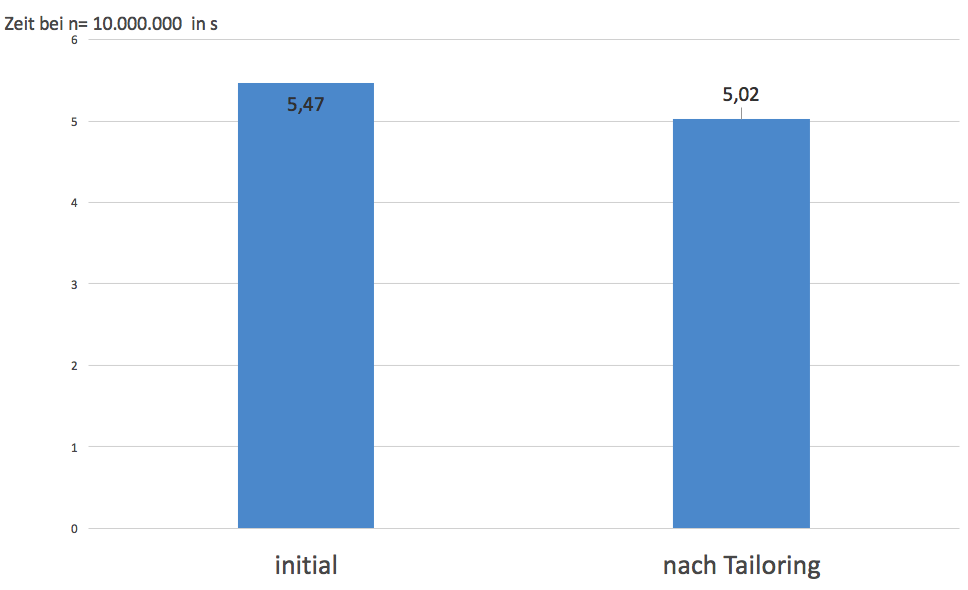
\includegraphics[width=0.6\columnwidth]{pro3fin} 
	\caption[Zusammenfassung Optimierung Alg. 3]{Zusammenfassung der Optimierung von Algorithmus 3}
\end{figure}\


\subsection{Wie wird gemessen?}
Mit den vorangegangen Kapiteln 5.1 - 5.3 soll die Optimierung der Implementierungen für das Projekt als abgeschlossen betrachtet werden. Eine ausführbare Implementierung für alle drei Algorithmen findet sich im Abgabeordner unter \textit{/05\_Finale\_Implementierung/}.\\ 
Nun sollen die Implementierungen dahingehend erweitert werden, um mit ihnen Zeitmessungen durchführen zu können.
Die Laufzeit wird dabei mithilfe der Funktion \textit{time() }des python-Moduls \textit{time} gemessen. Die Funktion \textit{time()} liefert die seit dem 1.1.1970 vergangene Zeit in Sekunden als Gleitkommazahl. \cite{TIME} Nach dem folgenden Schema wird somit die Laufzeit errechnet und in der Konsole ausgegeben.\\
\lstinputlisting[language=python]{pyCode2.py}\
Um mehrere Messungen für eine Messreihe mit steigendem \(n\) durchzuführen wird wie folgt verfahren.
\begin{enumerate}[noitemsep]
	\item Erzeugen der Ausgangsdaten per \textit{testDataGenerator.py} oder Java Anwendung \textit{realDataGetter}
	\item Erstellen mehrerer Playlists mit steigender Titelzahl \(n\) auf Grundlage der Ausgangsdaten mittels \textit{cutToLen.py} und \textit{shCutToLen.sh}
	\item Ausführen der zu untersuchenden Implementierung für alle generierten \textit{.txt}-Files mittes zuvor angepasstem shell-Skript \textit{shRunScript.sh}
\end{enumerate}\
Das shell-Skript \textit{shRunScript.sh} und die für die Laufzeit-Messungen angepassten Implementierungen sind im Abgabeordner unter \textit{/04\_Mess-Skripte/} enthalten.\\
Damit sind die Vorbereitungen für die Messungen abgeschlossen. In den folgenden Kapiteln sollen die untenstehenden Aspekte untersucht werden.
\begin{enumerate}[noitemsep]
		\item Vergleich der Laufzeit zwischen Echt- und Test-Daten.
		\item Abgleich der Laufzeit gegen die theoretische Laufzeit der Algorithmen.
		\item Grafischer Vergleich der Algorithmen untereinander.
		\item Durchführung statistischer Hypothesentests.
\end{enumerate}\


\section{Vergleich Echt vs. Test-Daten}
In diesem Kapitel sollen stichprobenartig die Laufzeiten der einzelnen Algorithmen beim Verarbeiten von Echt- und Test-Daten betrachtet werden. Dabei wird wie folgt verfahren.
\begin{enumerate}[noitemsep]
	\item Für drei verschiedene Ausgangs-Künstler mithilfe des Echt-Daten-Abgreifers Ausgangs-Playlists erzeugen.
	\item Mithilfe des Test-Daten-Generators drei Listen erstellen, wobei jede einer Echt-Daten-Liste in Länge und Dupikat-Faktor nachempfunden wird
	\item Einkürzen der drei Listen auf die Längen \(n=\{33.000,100.000,300.000\} \)
	\item Durchführen dreier Messungen pro Liste und Algorithmus.
\end{enumerate}\
Die unten dargestellten Graphen zeigen die aus den drei Messungen erzeugten Mittelwerte.\\
Der Vergleich für den Haupt-Algorithmus zeigt folgenden Graphen:
\begin{figure}[h!]
	\centering 
	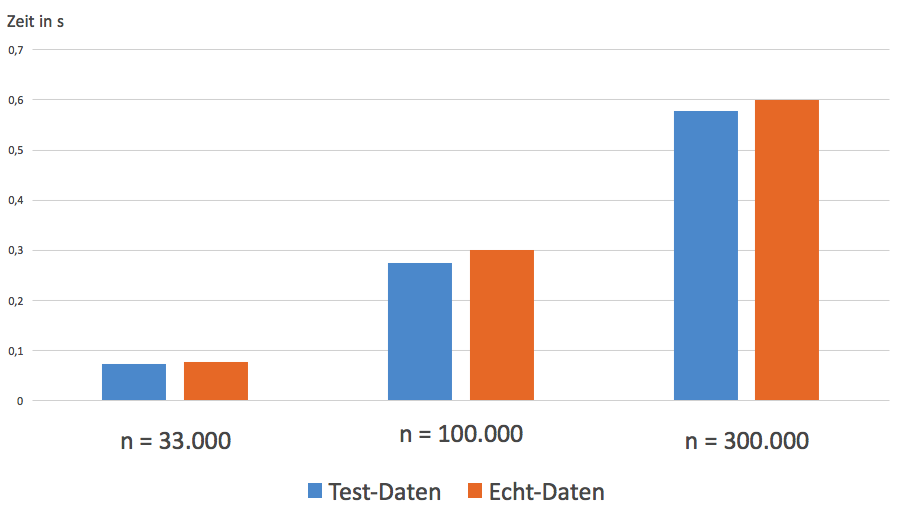
\includegraphics[width=0.7\columnwidth]{tr1} 
	\caption[Vergleich Echt- und Test-Daten für Alg.1]{Vergleich Echt- und Test-Daten für Algorithmus 1}
\end{figure}\

Die Graphen für die Vergleichs-Algorithmen zeigen ein ähnliches Bild.
\begin{figure}[h!]
	\centering 
	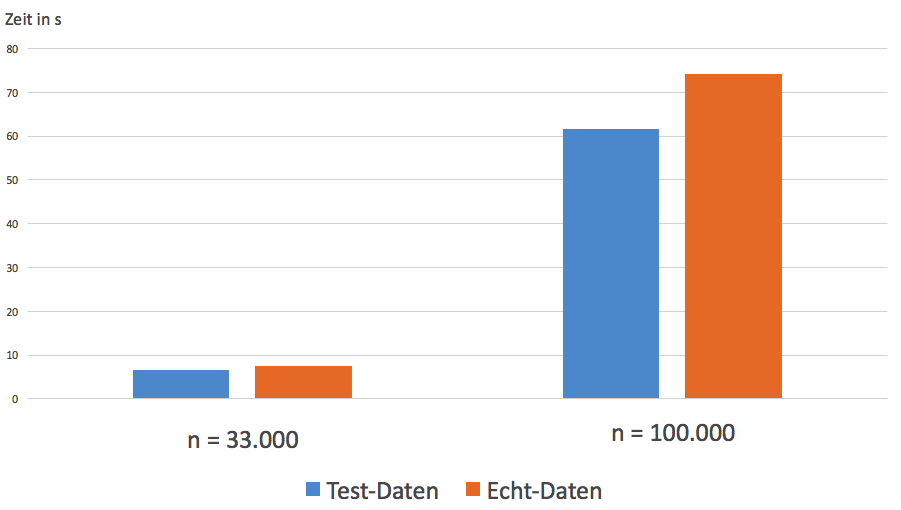
\includegraphics[width=0.7\columnwidth]{tr2} 
	\caption[Vergleich Echt- und Test-Daten für Alg.2]{Vergleich Echt- und Test-Daten für Algorithmus 2}
\end{figure}\
\begin{figure}[h!]
	\centering 
	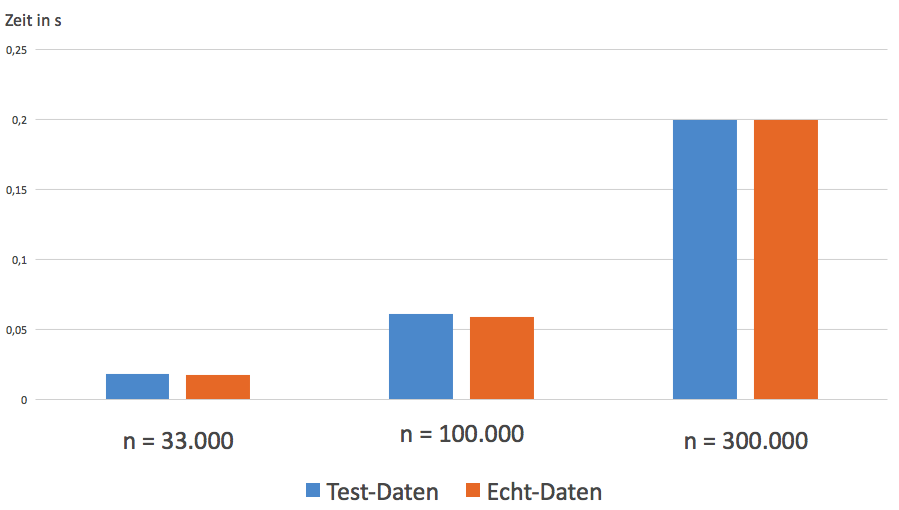
\includegraphics[width=0.7\columnwidth]{tr3} 
	\caption[Vergleich Echt- und Test-Daten für Alg.3]{Vergleich Echt- und Test-Daten für Algorithmus 3}
\end{figure}\

Es lässt sich festhalten, dass sich die Laufzeiten für alle drei Algorithmen zumindest für die vorgenommenen Stichproben nicht signifikant voneinander unterscheiden. Eventuelle erkennbare Unterschiede, wie das abweichen der Laufzeiten für \(n=100.000\) in Algorithmus 2 könnten mit weiteren Laufzeitmessungen untersucht werden. Für die Projektarbeit soll dieser Verglich jedoch genügen.\\ 
Für alle folgenden Messungen sollen Echt-Daten verwendet werden.
\pagebreak
\section{Vergleich mit theoretischer Laufzeit}
Um pro Algorithmus den Vergleich mit der theoretischen Laufzeit anzustellen, werden pro Algorithmus folgende Laufzeitmessungen durchgeführt:
\begin{itemize}[noitemsep]
	\item Pro Messreihe: Playlists mit aufsteigender Titel-Anzahl \(n = \{5000,10.000,...,100.000\}\)
	\item Durchführung von 9 Messreihen:
	\subitem Für drei verschiedene Playlists mit unterschiedlichem Ausgangs-Künstler
	\subsubitem Durchführen dreier Messungen pro Echt-Daten-Playlist.
\end{itemize}\
Die Messergebisse werden zunächst in einem Boxplot-Diagramm dargestellt. Zur Überprüfung der theoretischen Laufzeit wird die y-Achse des Diagrammes entsprechend der jeweiligen theoretischen Laufzeit skaliert.

\subsection{Haupt-Algorithmus}
Das Boxplot-Diagramm für den Haupt-Algorithmus zeigt das folgende Bild:
\begin{figure}[h!]
	\centering 
	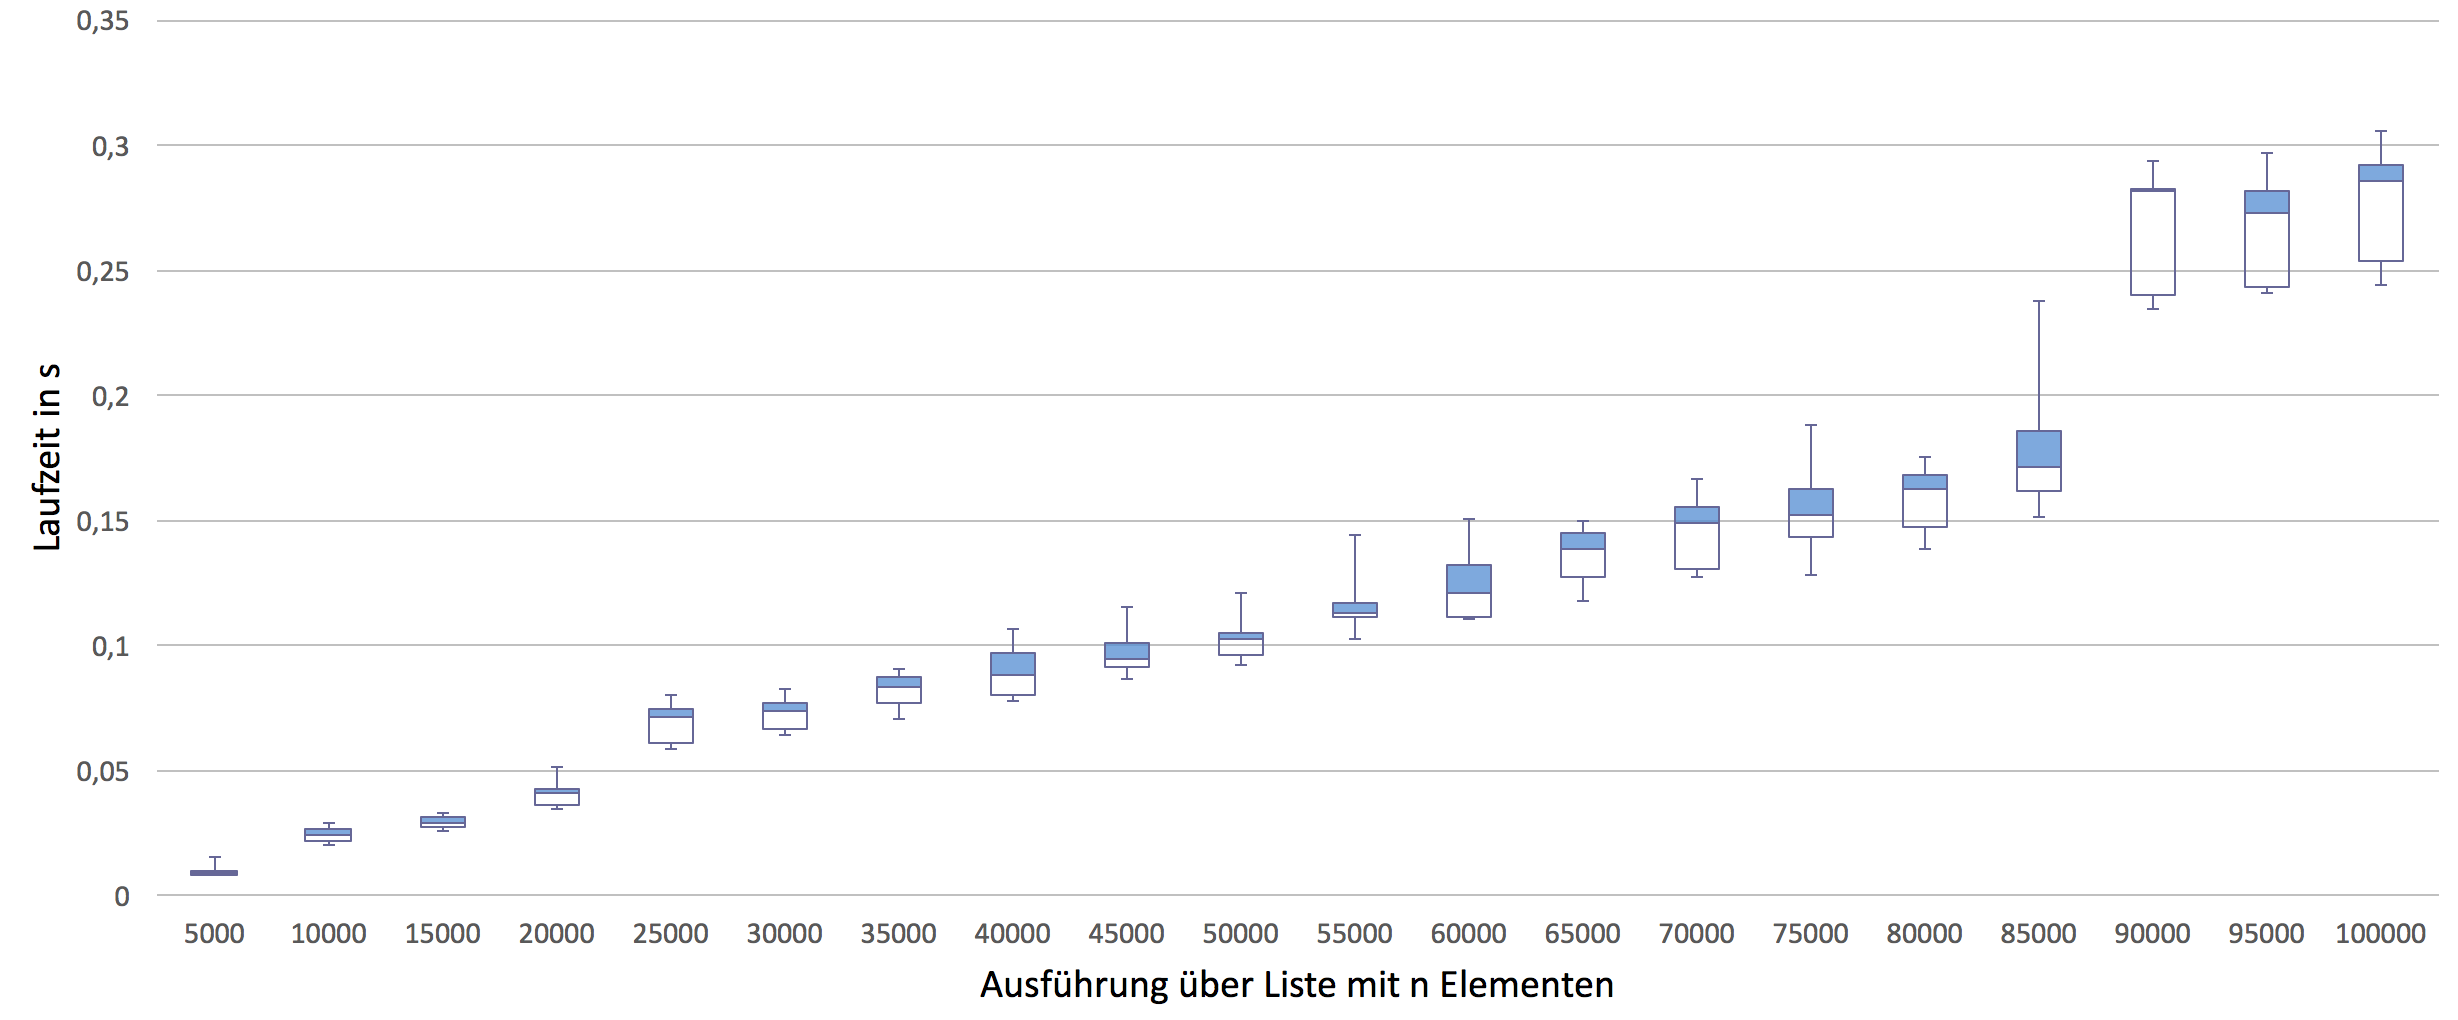
\includegraphics[width=\columnwidth]{bp1} 
	\caption[Darstellung Laufzeitmessungen Alg. 1 im Boxplot-Diagramm]{Darstellung der Laufzeitmessungen für Algorithmus 1 im Boxplot-Diagramm}
\end{figure}\

Wird dieser mit der in Kapitel 1 beschriebenen theoretischen Laufzeit von \(O=(n)\) skaliert, zeigt sich das folgende Bild:

\begin{figure}[h!]
	\centering 
	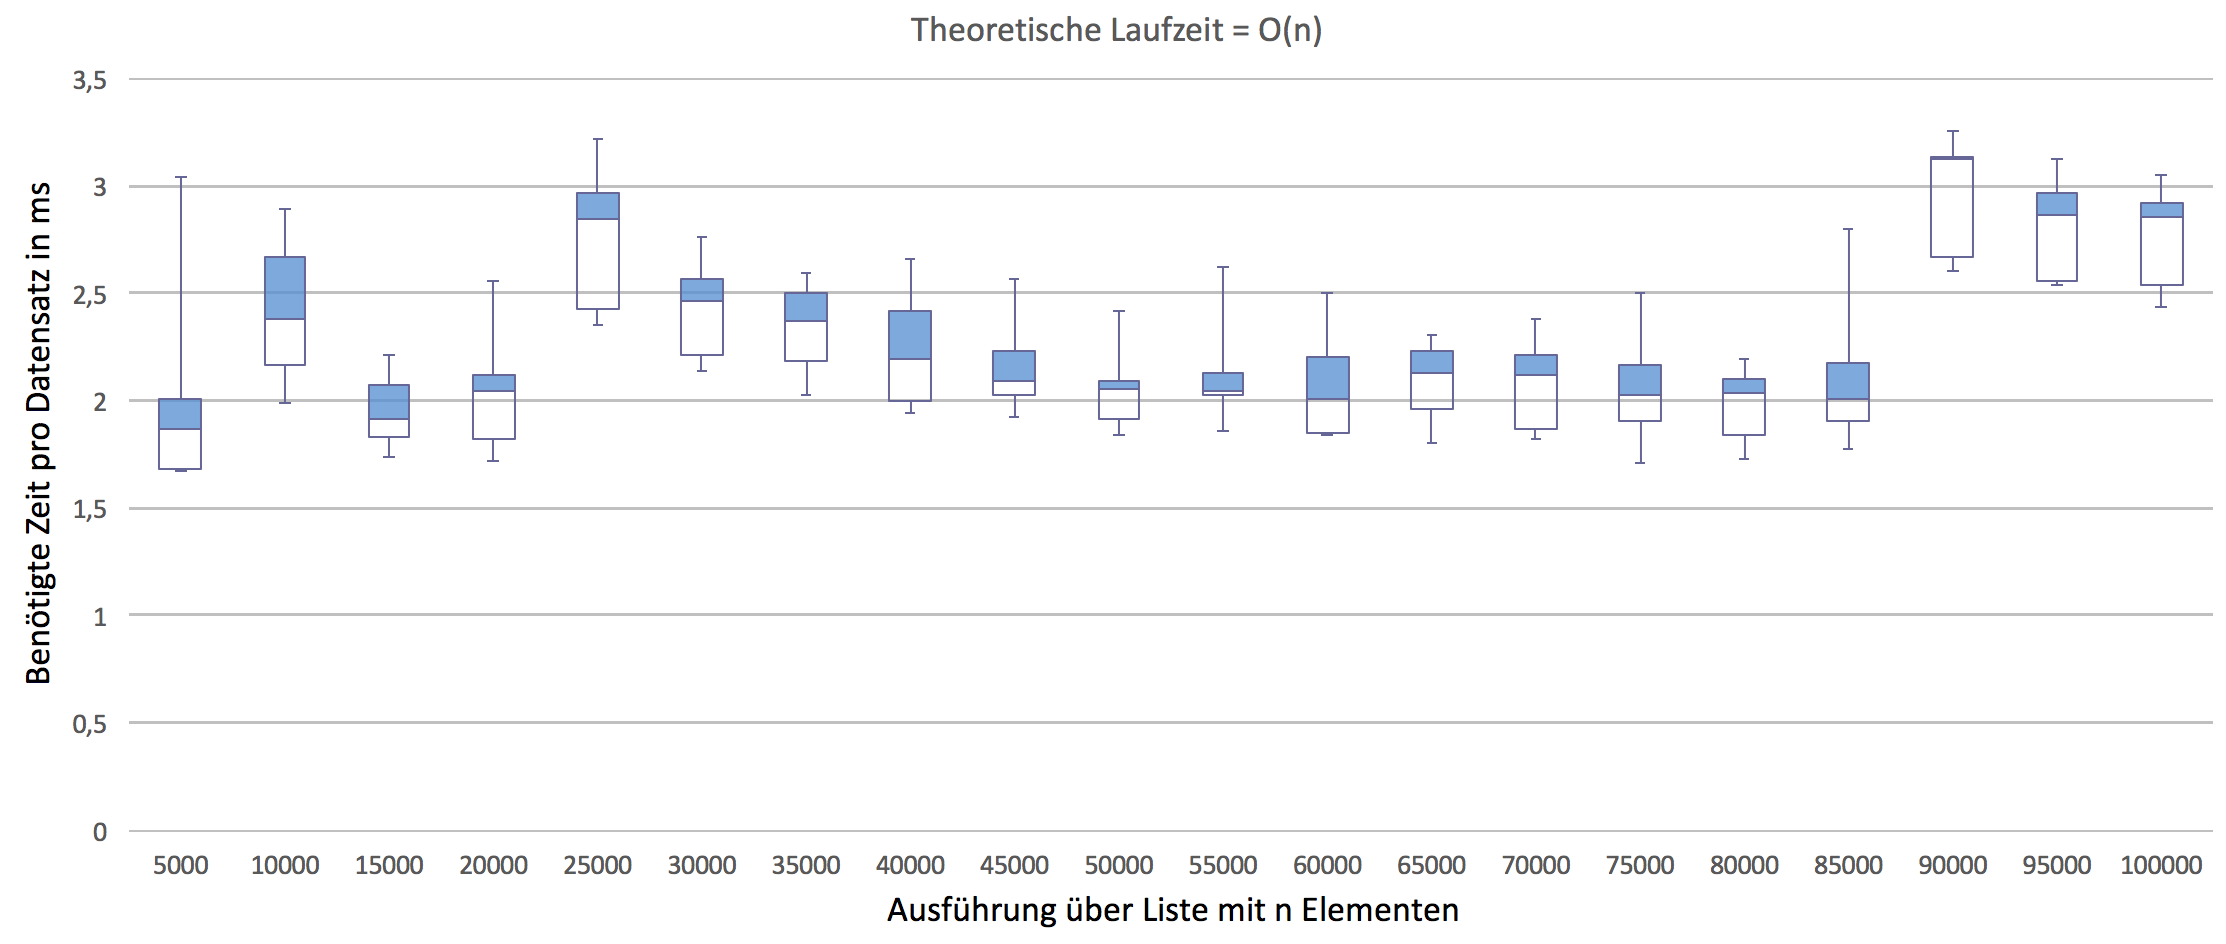
\includegraphics[width=\columnwidth]{bp2} 
	\caption[]{Laufzeitmessungen für Algorithmus 1 im skalierten Boxplot-Diagramm}
\end{figure}\

Es wird ersichtlich, dass die Laufzeiten pro Datensatz nahezu in einer Geraden liegen, was die theoretische Laufzeit bestätigt. \\
Es lässt sich jedoch ein leichter Anstieg der Geraden erkennen. Der Grund dafür zeigt sich im unskalierten Boxplot-Diagramm. In diesem ist ein sprunghafter Anstieg der Laufzeit für die n-Werte \(n=25.000\) und \(n=90.000\) zu abzulesen. Als Ursache dafür lässt sich wiederum das Kopieren aller Werte der hash-table in die neu angelegte, vergrößerte hash-table vermuten \textit{(Siehe Kapitel 3.1 - Haupt-Algorithmus: Elemente in Array einfügen, Zeilen 32-29)}
\subsection{Vergleichs-Algorithmus 1}
Für den Vergleichs-Algorithmus 1 zeigt das Ausgangs-Boxplot-Diagramm und das mit der in Kapitel 1 hergeleiteten theoretischen Laufzeit von \(O=(n^2)\) skalierte Diagramm, dass die Laufzeit-Überlegung als bestätigt betrachtet werden kann.
\begin{figure}[h!]
	\centering 
	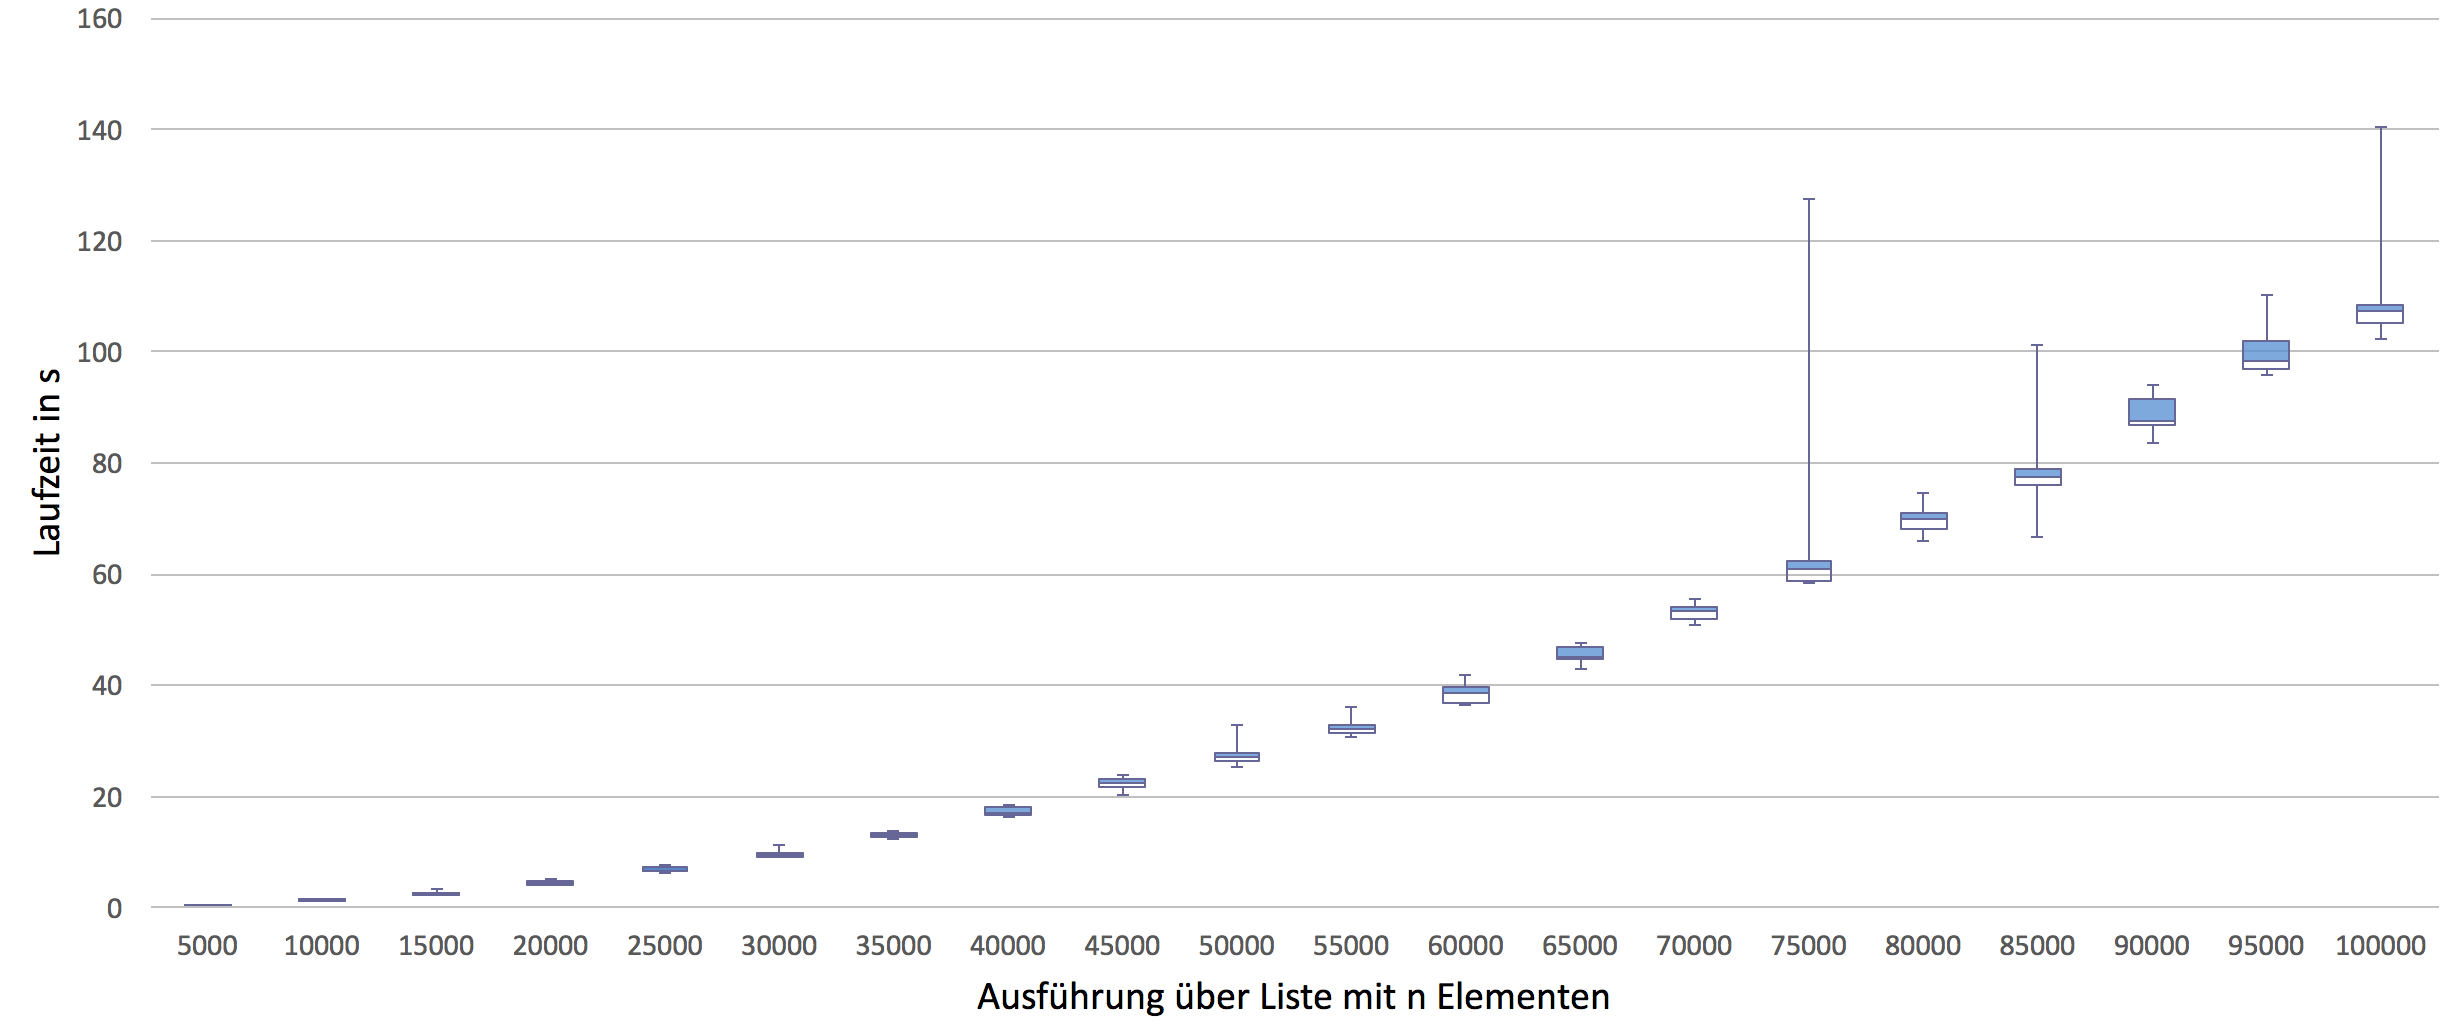
\includegraphics[width=\columnwidth]{bp3} 
	\caption[]{Darstellung der Laufzeitmessungen für Algorithmus 2 im Boxplot-Diagramm}
\end{figure}\
\begin{figure}[h!]
	\centering 
	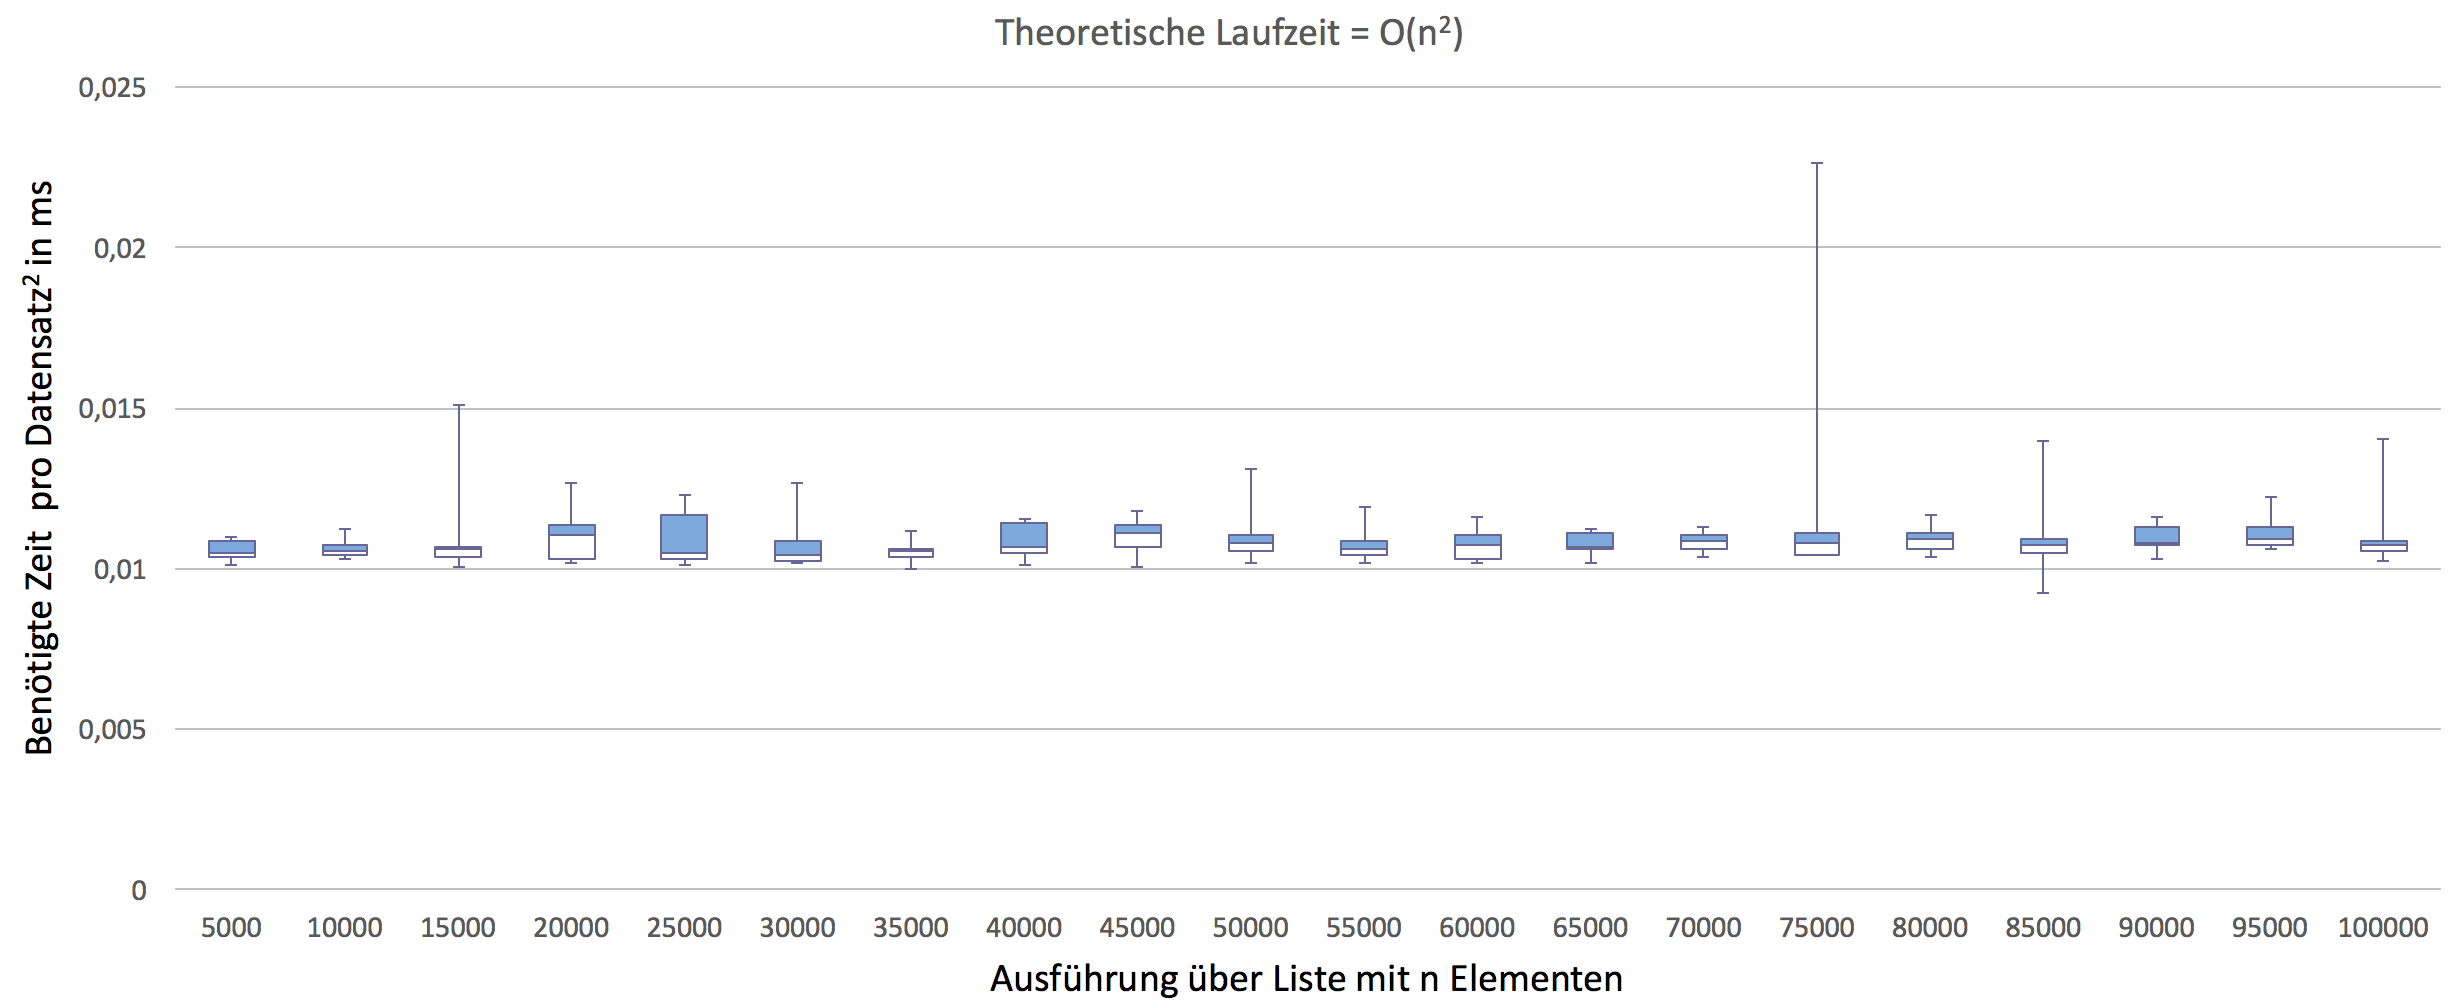
\includegraphics[width=\columnwidth]{bp4} 
	\caption[]{Laufzeitmessungen für Algorithmus 2 im skalierten Boxplot-Diagramm}
\end{figure}\


\subsection{Vergleichs-Algorithmus 2}
Die Betrachtung der Laufzeiten in den entsprechenden Diagrammen für den dritten Algorithmus, zeigen, dass auch hier die theoretische Laufzeit bestätigt werden kann. Der für den Haupt-Algorithmus festgestellte sprunghafte Anstieg der Laufzeit für \(n=25.000\) und \(n=90.000\) wird ebenfalls, wenn auch sehr viel dezenter, ersichtlich.
\pagebreak
\begin{figure}[h!]
	\centering 
	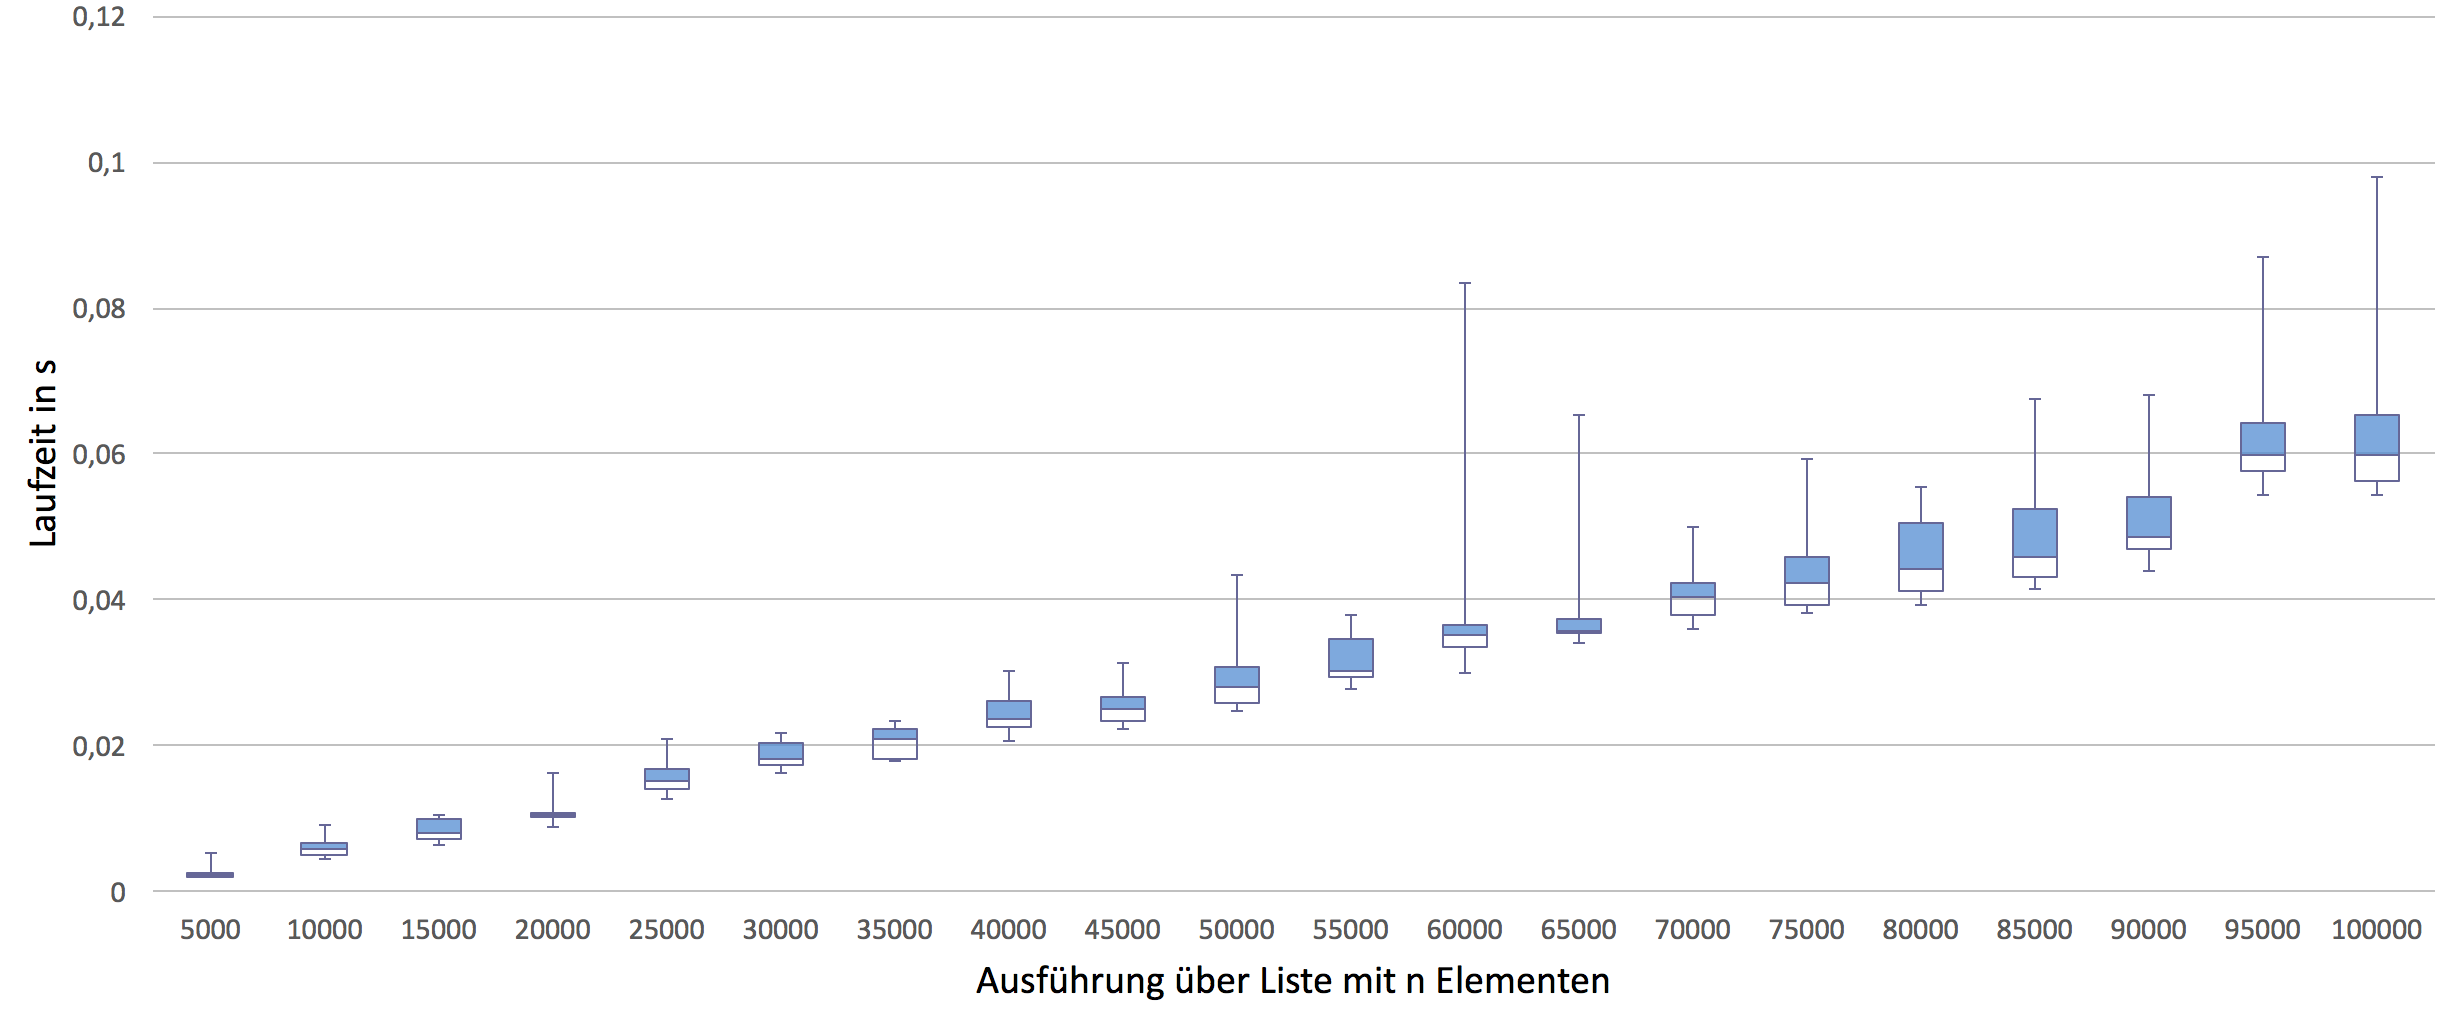
\includegraphics[width=\columnwidth]{bp5} 
	\caption[]{Darstellung der Laufzeitmessungen für Algorithmus 3 im Boxplot-Diagramm}
\end{figure}\
\begin{figure}[h!]
	\centering 
	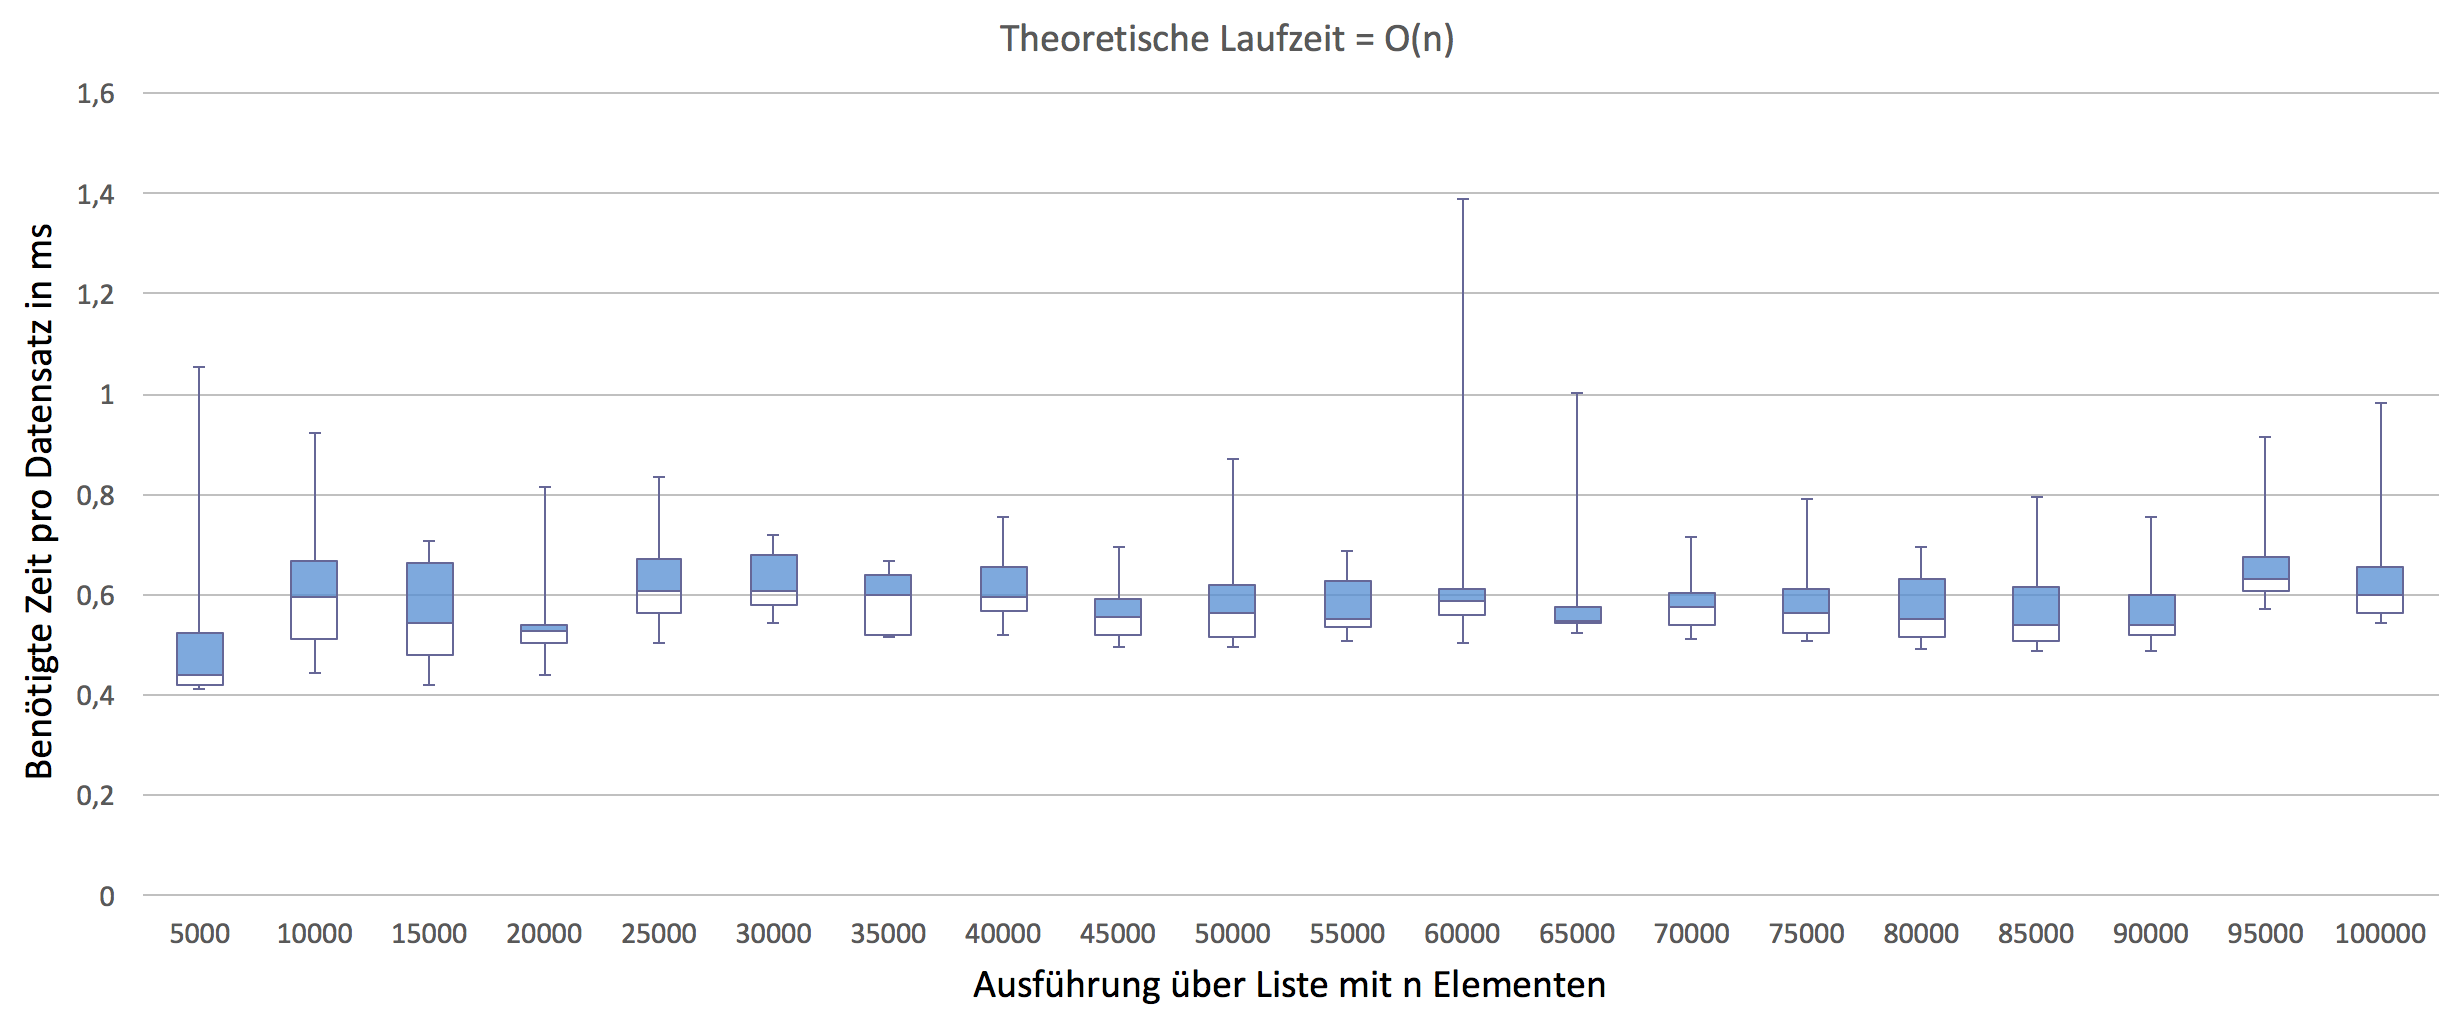
\includegraphics[width=\columnwidth]{bp6} 
	\caption[]{Laufzeitmessungen für Algorithmus 3 im skalierten Boxplot-Diagramm}
\end{figure}\
\pagebreak
\section{Vergleich der Algorithmen}
\subsection{Grafischer Vergleich}
Für den grafischen Vergleich der Algorithmen-Laufzeiten untereinander, werden für allen drei Algorithmen Laufzeitmessung für die folgenden Probleminstanzen durchgeführt:
\begin{itemize}[noitemsep]
	\item Für mehrere Playlists mit wachsende Titel-Anzahl \(n = \{20,40,...,1000\}\)
	\subitem Pro \(n\): 10 verschiedene Echtdaten-Tracklisten
	\subsubitem Pro Liste: 3 Messdurchläufe
\end{itemize}\
Die Messreihen wurden über das Ablehnen von Messungen außerhalb des Bereiches \([\mu-\sigma,\mu+\sigma]\) bereinigt, wobei \(\mu\) der Erwartungswert und \(\sigma\) die Standardabweichung der Messwerte ist.\\
Der direkte grafische Vergleich stellt sich wie folgt dar.\\
\begin{figure}[h!]
	\centering 
	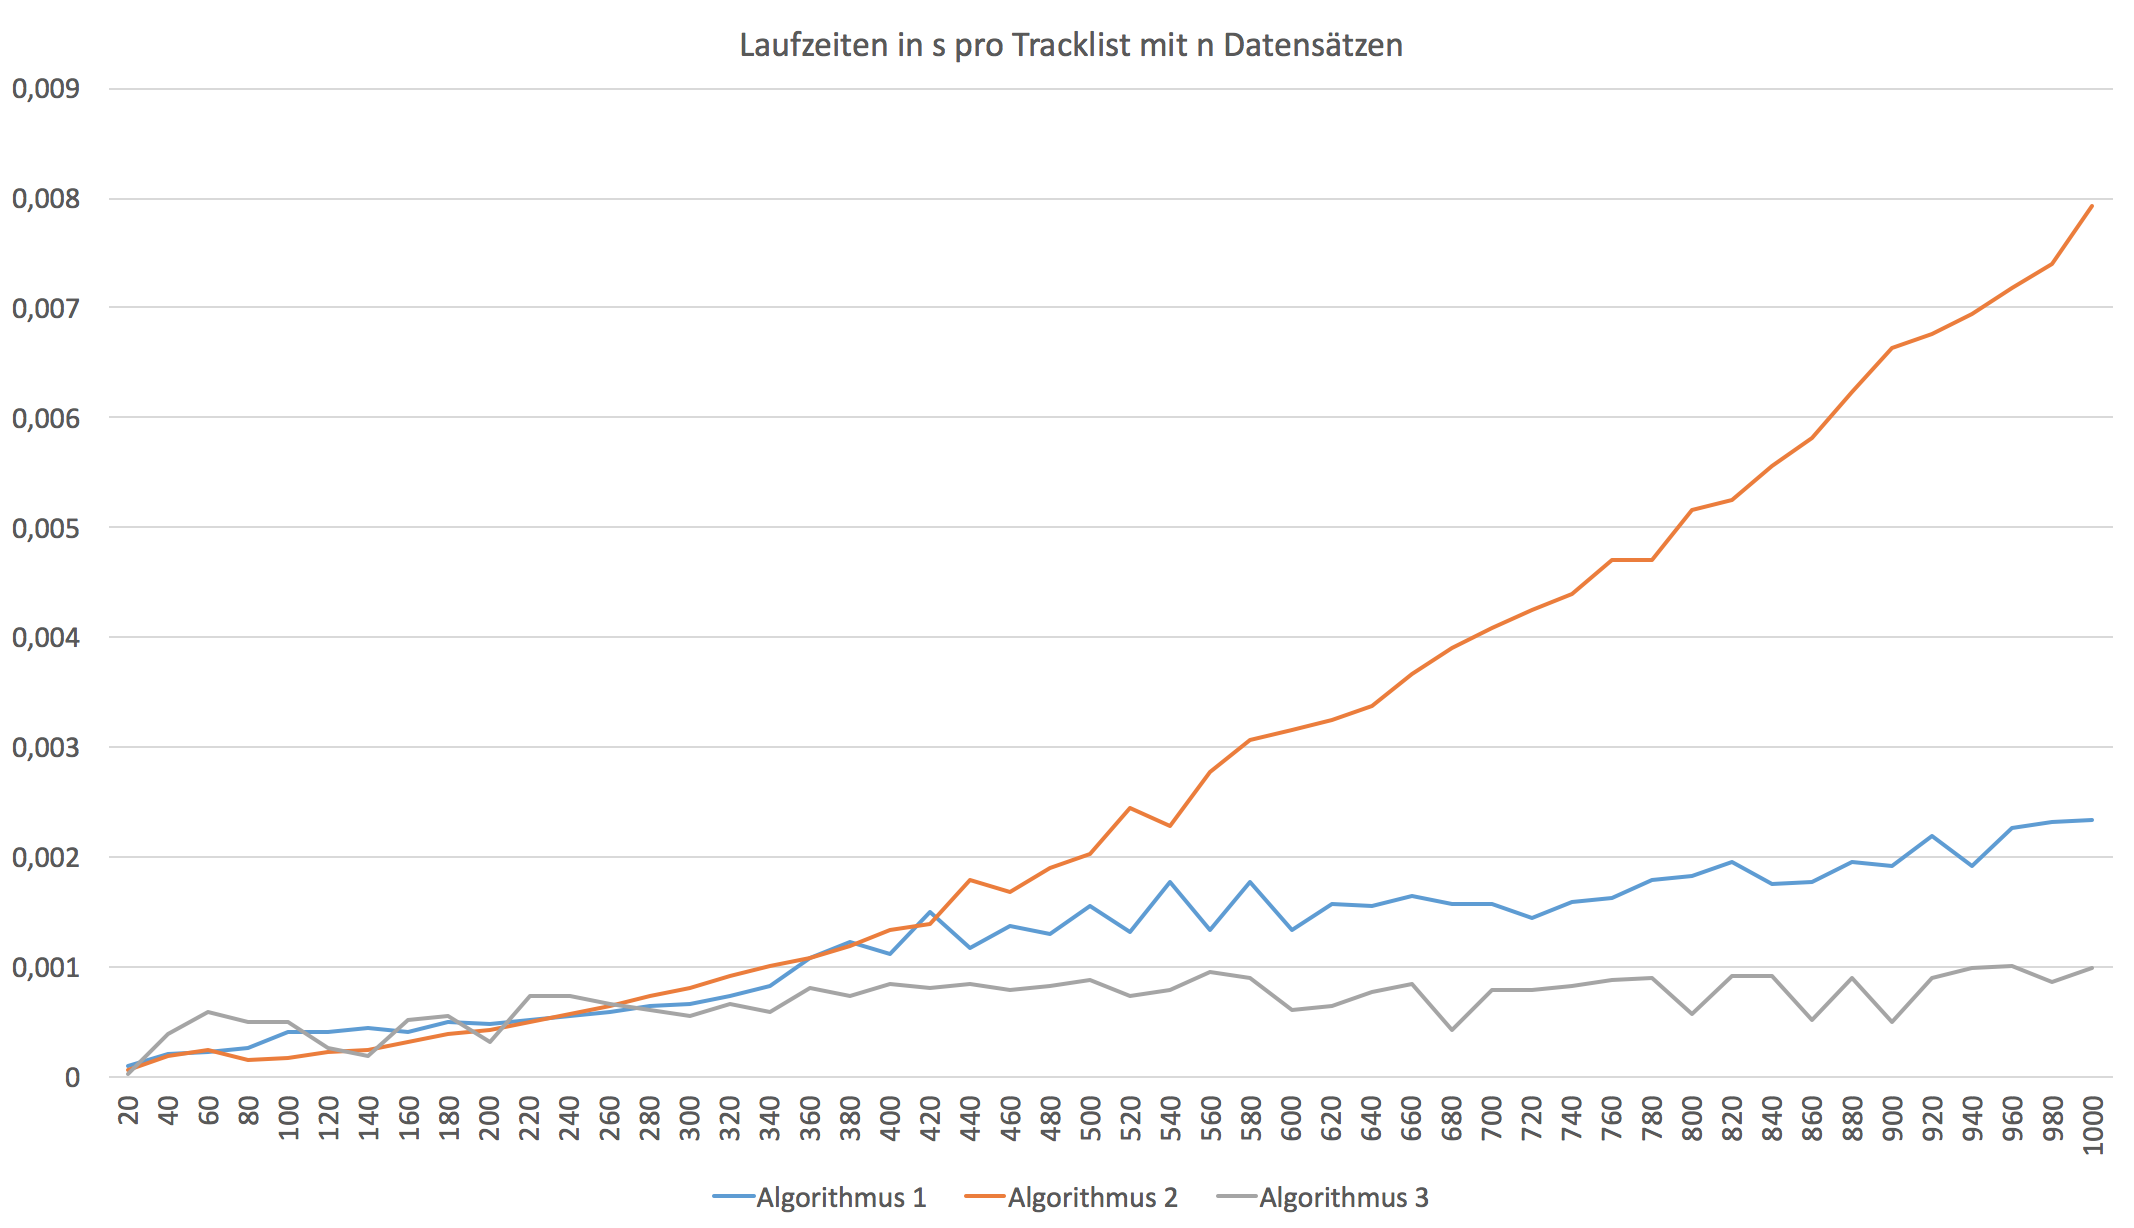
\includegraphics[width=\columnwidth]{compare1} 
	\caption[]{Direkter grafischer Vergleich der Algorithmen miteinander}
\end{figure}\
Die Laufzeit für Algorithmus 2 nimmt, wie in der Betrachtung der theoretischen Laufzeit bestätigt exponentiell zu. Um jedoch einen besseren Eindruck für das Laufzeitverhalten von Algorithmus 1 und algorithmus 3 zu gewinnen, wird für diese ein weiterer Vergleich mit höheren \(n\)-Werten angestellt:\\
\begin{itemize}[noitemsep]
	\item Für mehrere Playlists mit wachsende Titel-Anzahl \(n = \{2000,4000,...,100.000\}\)
	\subitem Pro \(n\): 10 verschiedene Echtdaten-Tracklisten
	\subsubitem Pro Liste: 3 Messdurchläufe
\end{itemize}
In diesem Vergleich wird die Relation der Laufzeiten deutlich. Ebenfalls sind für beide Implementierungen die in Kapitel 7.1 festgestellten sprunghaften Anstiege der Laufzeiten aufgrund der hash-Tabellen-Kopier-Operationen festzustellen.
\pagebreak
\begin{figure}[h!]
	\centering 
	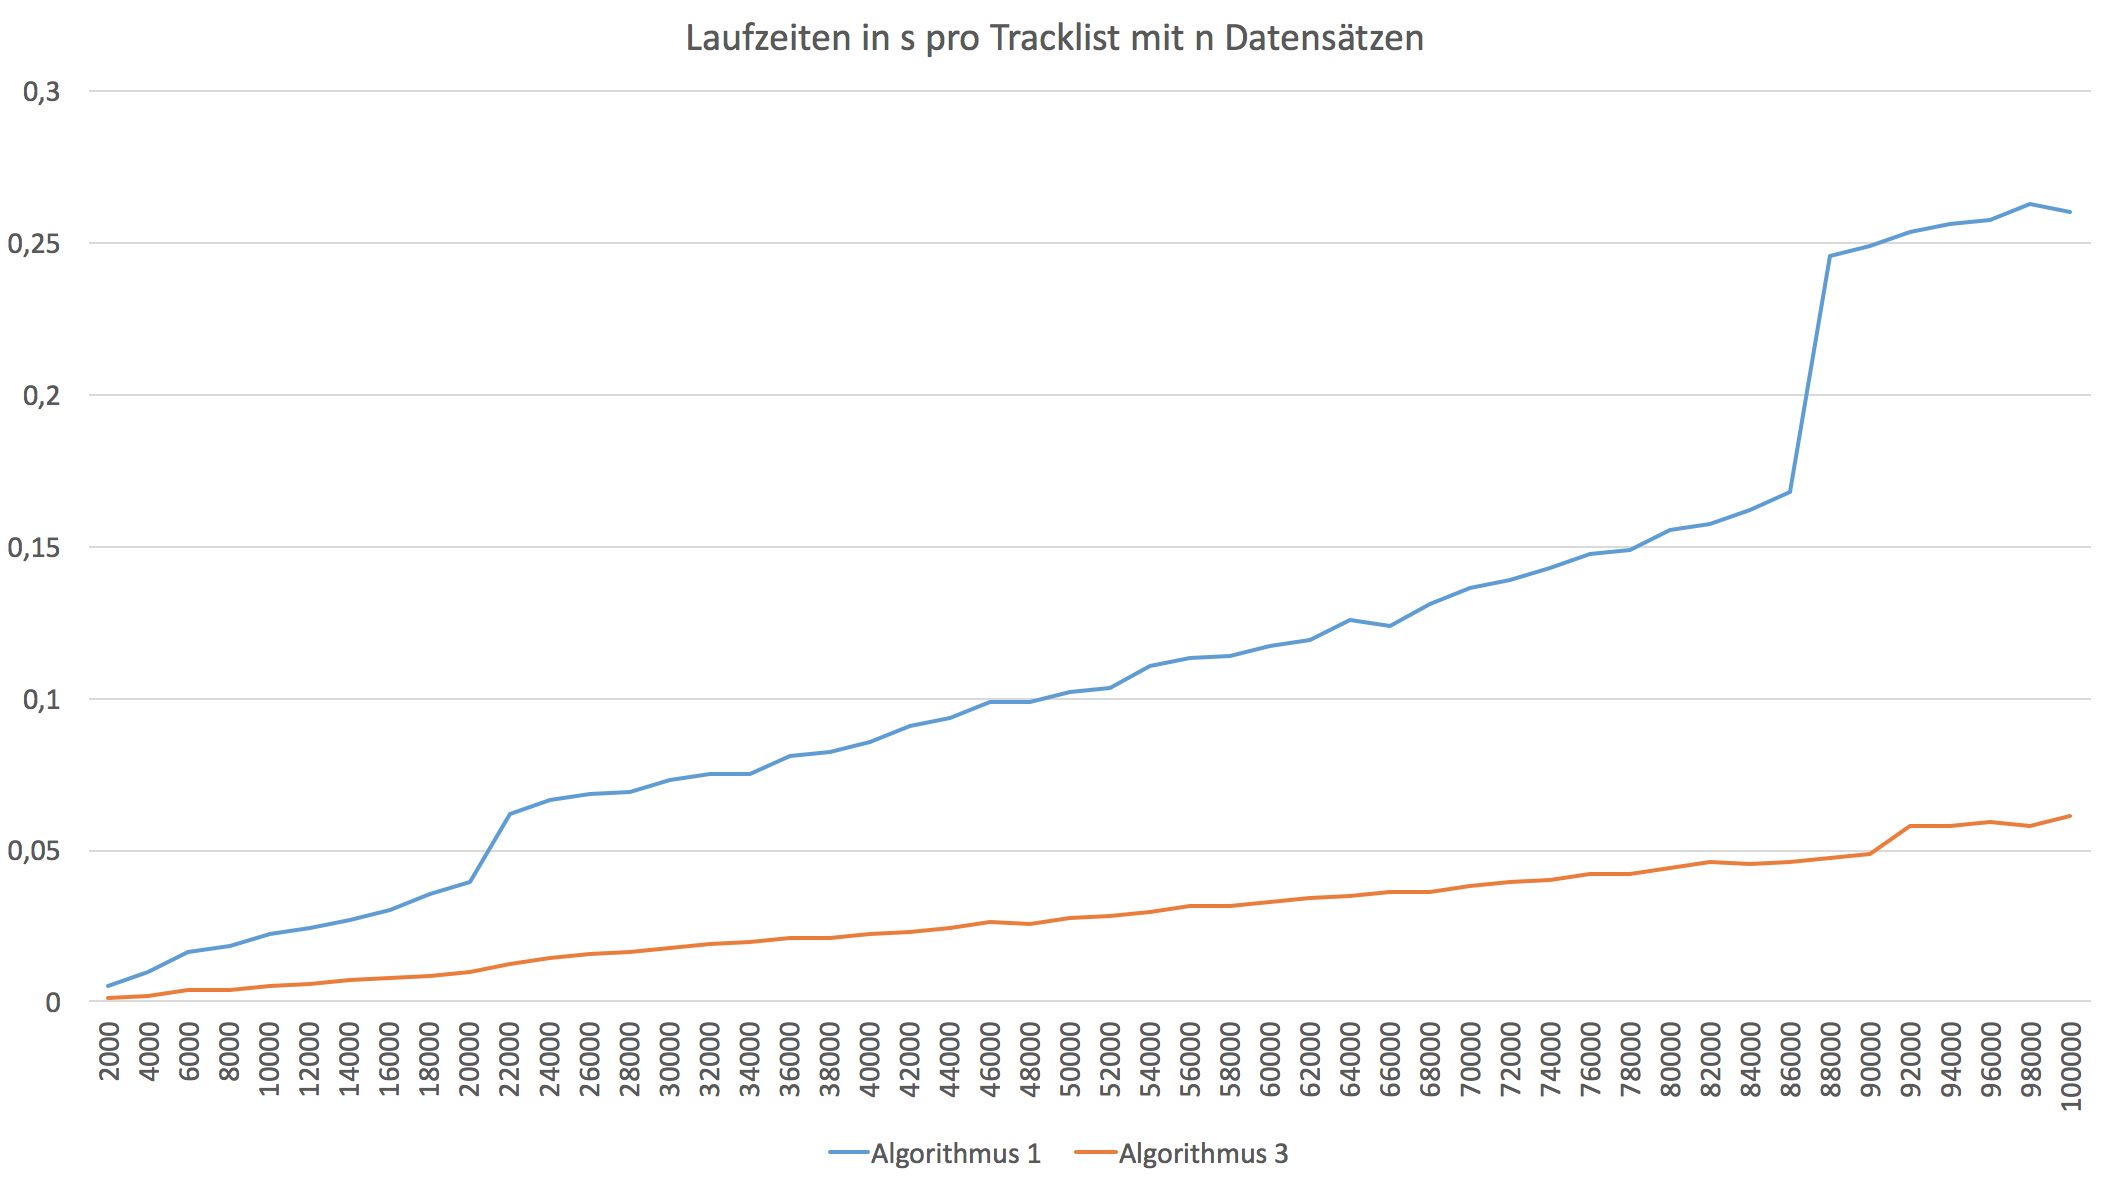
\includegraphics[width=\columnwidth]{compare2} 
	\caption[]{Direkter grafischer Vergleich der Algorithmen 1 und 3 miteinander}
\end{figure}\
Insgesamt lässt sich aus der grafischen Betrachtung die folgende Ordnung der Algotithmen-Laufzeiten anzunehmen.\\
\begin{equation}
Alg3_{Laufzeit} < Alg1_{Laufzeit} < Alg2_{Laufzeit}
\end{equation}\

\subsection{Statistischer Hypothesen-Test}
Auf Grundlage der im vorherigen Kapitel durchgeführten Messungen für \(n = \{20,40,...,1000\}\) soll nun eine exakte Analyse mittels statistischer Hypothesentests durchgeführt werden. Dabei soll die angestellte Überlegung\\
\begin{equation}
Alg3_{Laufzeit} < Alg1_{Laufzeit} < Alg2_{Laufzeit}
\end{equation}\
als Ausgangspunkt verwendet werden.\\ Um zu überprüfen, ab welcher Playlist-Größe die einzelnen Teile der Relation sicher gelten, sollen durch die folgenden Hypothesentests drei Aussagen geprüft werden:
\begin{enumerate}[noitemsep]
	\item Algorithmus 1 ist schneller als Algorithmus 2
	\item Algorithmus 3 ist schneller als Algorithmus 2
	\item Algorithmus 3 ist schneller als Algorithmus 1
\end{enumerate}\

\textbf{Algorithmus 1 schneller als Algorithmus 2}\\
Aus der Vermutung, dass Algorithmus 1 schneller ist, als Algorithmus 2 ergeben sich für den linksseitigen Hypothesentest die Null-Hypothese 
\begin{equation}
H_0: \tilde{ \mu_1 } \ge \tilde{\mu_2}
\end{equation}\
und die Alternativ-Hypothese
\begin{equation}
 H_0: \tilde{ \mu_1 } < \tilde{\mu_2}
\end{equation}\
wobei \(\tilde{ \mu}\) je den Mittelwerten aller Messungen für eine Probleminstanz entspricht.\\
Nun soll überprüft werden, ob die Nullhypothese pro \(n\) bestätigt werden kann oder zu widerlegen ist. Dabei soll ein frei gewähltes Signifikanzniveau von \(\alpha = 0,02\%\)  verwendet werden.\\
Über die Differenzen aller Messwerte \(d_i = MesswertAlg2_i - MesswertAlg1_i\) werden dazu der Erwartungswert \(\mu_d\) und die Standardabweichung \(\sigma_d \) ermittelt. Auf dieser Grundlage wird der t-Wert \(t=\sqrt{n}\frac{\mu_d}{\sigma_d} \) ermittelt und mit dem Wert der t-Funktion für \(t(0,98;29)\approx2,15\) verglichen.\\
Die Nullhypothese ist dabei abzulehnen, wenn gilt \(t<2,15\)\\
Das Resultat gestaltet sich wie folgt:
\begin{table}[h!]
	\centering 
	\begin{tabular}{|l|c|c|c|c|}
	\hline
				n   &		\(t=\sqrt{n}\frac{\mu_d}{\sigma_d} \)				& \(t(0,98;29)\) &	Ergebnis\\
	\hline
	20   	&	-4,675596311	& 2,15 &	Null-Hypothese nicht abgelehnt\\
	\hline
	40   	&	-2,267865616	& 2,15 &	Null-Hypothese nicht abgelehnt\\
	\hline
	60...380   &		...			  & 2,15 &		Null-Hypothese nicht abgelehnt\\
	\hline
	400   &		1,551055352   &	 2,15 &	Null-Hypothese nicht abgelehnt\\
	\hline
	420   &		0,540433623   &	 2,15 &	Null-Hypothese nicht abgelehnt\\
	\hline
	440   &		4,598993754   &	 2,15 &	Null-Hypothese abgelehnt\\
	\hline
	460   &		3,17978148    &	 2,15 &	Null-Hypothese abgelehnt\\
	\hline
	480...980   &		...			  &	 2,15 &	Null-Hypothese abgelehnt\\
	\hline
	1000   &		35,12686104	&  2,15 &	Null-Hypothese abgelehnt\\
	\hline
	\end{tabular}\\
	\caption[]{Ergebnisse Hypothesentest ''Algorithmus 1 schneller als Algorithmus 2''}
\end{table}\

Folglich, kann bei einem angenommenen Signifikanzniveau von \(\alpha = 0,02\%\) erst ab einer Playlistgröße von \(n = 440\) angenommen werden, dass Algorithmus 1 eine geringere Laufzeit hat, als Algorithmus 2.\\

\textbf{Algorithmus 3 schneller als Algorithmus 2}\\
Das Verfahren für den linksseitigen Hypothesentest ist dem obigen analog.\\
Es gelten Null-Hypothese:
\begin{equation}
H_0: \tilde{ \mu_3 } \ge \tilde{\mu_2}
\end{equation}\
und Alternativ-Hypothese
\begin{equation}
H_0: \tilde{ \mu_3 } < \tilde{\mu_2}
\end{equation}\
Das oben genutzte Signifikanzniveau von \(\alpha = 0,02\%\) soll auch hier angewendet werden. Es ergibt sich die folgende Tabelle:
\begin{table}[h!]
	\centering 
	\begin{tabular}{|l|c|c|c|c|}
		\hline
		n   &		\(t=\sqrt{n}\frac{\mu_d}{\sigma_d} \)				& \(t(0,98;29)\) &	Ergebnis\\
		\hline
		20   	&	4,184966485	& 2,15 &	Null-Hypothese abgelehnt\\
		\hline
		40   	&	-4,405691129	& 2,15 &	Null-Hypothese nicht abgelehnt\\
		\hline
		60...280   &		...			  & 2,15 &		Null-Hypothese nicht abgelehnt\\
		\hline
		300   &		1,822671007   &	 2,15 &	Null-Hypothese nicht abgelehnt\\
		\hline
		320   &		2,486409842   &	 2,15 &	Null-Hypothese abgelehnt\\
		\hline
		340...980   &		...			  &	 2,15 &	Null-Hypothese abgelehnt\\
		\hline
		1000   &		39,26755684	&  2,15 &	Null-Hypothese abgelehnt\\
		\hline
	\end{tabular}\\
	\caption[]{Ergebnisse Hypothesentest ''Algorithmus 3 schneller als Algorithmus 2''}
\end{table}\

Folglich, kann bei einem angenommenen Signifikanzniveau von \(\alpha = 0,02\%\) erst ab einer Playlistgröße von \(n = 320\) und für die untersuchte Größe \(n = 20\) angenommen werden, dass Algorithmus 3 eine geringere Laufzeit hat, als Algorithmus 2.\\

\textbf{Algorithmus 3 schneller als Algorithmus 1}\\
Diese Untersuchung erfolgt analog der zwei vorangegangenen.\\
Es gelten Null-Hypothese:
\begin{equation}
H_0: \tilde{ \mu_3 } \ge \tilde{\mu_1}
\end{equation}\
und Alternativ-Hypothese
\begin{equation}
H_0: \tilde{ \mu_3 } < \tilde{\mu_1}
\end{equation}\
Das oben genutzte Signifikanzniveau von \(\alpha = 0,02\%\) soll weiterhin angewendet werden. Es ergibt sich die folgende Tabelle:

\begin{table}[h!]
	\centering 
	\begin{tabular}{|l|c|c|c|c|}
		\hline
		n   &		\(t=\sqrt{n}\frac{\mu_d}{\sigma_d} \)				& \(t(0,98;29)\) &	Ergebnis\\
		\hline
		20   	&	7,690375185	& 2,15 &	Null-Hypothese abgelehnt\\
		\hline
		40   	&	-2,382882348	& 2,15 &	Null-Hypothese nicht abgelehnt\\
		\hline
		60...180   	&	...	& 2,15 &	Null-Hypothese nicht abgelehnt\\
		\hline
		180   &			-0,568085214		  & 2,15 &		Null-Hypothese nicht abgelehnt\\
		\hline
		200   &		2,239280659  &	 2,15 &	Null-Hypothese abgelehnt\\
		\hline
		220   &	0,059793204	   &	 2,15 &	Null-Hypothese nicht abgelehnt\\
		\hline
		240...280   &		...			  &	 2,15 &	Null-Hypothese nicht abgelehnt\\
		\hline
		300   &		1,338695858	&  2,15 &	Null-Hypothese nicht abgelehnt\\
		\hline
		320   &		2,243603114	&  2,15 &	Null-Hypothese abgelehnt\\
		\hline
		340...980   &		...	&  2,15 &	Null-Hypothese abgelehnt\\
		\hline
		1000   &	8,43624219	&  2,15 &	Null-Hypothese abgelehnt\\
		\hline
	\end{tabular}\\
	\caption[]{Ergebnisse Hypothesentest ''Algorithmus 3 schneller als Algorithmus 1'}
\end{table}\

Es kann also bei einem angenommenen Signifikanzniveau von \(\alpha = 0,02\%\) erst ab einer Playlistgröße von \(n = 320\) sowie für die untersuchten Größen \(n = 20\)  und \(n = 200\) angenommen werden, dass Algorithmus 3 eine geringere Laufzeit hat, als Algorithmus 1.\\

\section{Fazit}

Neben dem erlangen von Kenntnissen über das Durchführen von Laufzeituntersuchungen zieht der Autor dieser Arbeit den folgenden Schluss:

\begin{quotation}
	''Wenn schon python, dann Standard-Funktionalitäten verwenden.''
\end{quotation}

\pagebreak

%----------------------------------------------------------------------------------------
%	BIBLIOGRAPHY
%----------------------------------------------------------------------------------------

\renewcommand{\refname}{\spacedlowsmallcaps{Literatur/Quellen}} % For modifying the bibliography heading

\bibliographystyle{unsrt}

\bibliography{bib.bib} % The file containing the bibliography

%----------------------------------------------------------------------------------------

\end{document}